
\pdfminorversion=4
\documentclass[letterpaper,12pt]{article}
\usepackage[top=1in, bottom=1in, left=1.25in, right=1.25in]{geometry}
\usepackage{setspace}
\setcounter{secnumdepth}{3} % this number depends on your depth of sections
\setcounter{tocdepth}{3} % this number should be equal to secnumdepth in previous
%\usepackage{subfigure}
%\usepackage[subfigure]{tocloft}
\usepackage{subcaption}
\usepackage{tocstyle}
\renewcommand{\contentsname}{\centerline {\normalsize\bfseries Table of Contents}}
\newtocstyle[standard][leaders]{mytocstyle}{\settocfeature[1]{entryhook}{\normalfont\bfseries}}
\usepackage[capposition=top]{floatrow}
\usepackage{listings}
\usepackage{cite}
\usepackage{footnote}
\usetocstyle{mytocstyle}
\usepackage{sectsty}
\sectionfont{\normalsize\centering}
\subsectionfont{\normalsize}
\usepackage{enumitem}
\renewcommand{\thesection}{}
\renewcommand{\thesubsection}{\arabic{section}.\arabic{subsection}}
\usepackage{algorithmicx}
\usepackage{algorithm}
\usepackage{algpseudocode}
\usepackage{algpascal}
\usepackage{algc}
\usepackage{graphicx}
\usepackage{times}
\usepackage{latexsym}
\usepackage{graphicx}
\usepackage{cite}
\usepackage{balance}
\usepackage{multirow}
\usepackage{epstopdf}
\usepackage{threeparttable}
\usepackage[latin1]{inputenc}
\usepackage{amsmath}
\usepackage{amsfonts}
\usepackage{amssymb}
\usepackage{amsthm}
%\usepackage{algorithm}
%\usepackage{algorithmic}
\graphicspath{ {images/} }
\usepackage{graphicx}
\usepackage{comment}
\usepackage{times}
\usepackage{cite}
\newtheorem{theorem}{Theorem}
\newtheorem{lemma}{Lemma}
\newtheorem{definition}{Definition}
\newenvironment{alginc}[1][pseudocode]{\medskip\algsetlanguage{#1}\begin{algorithmic}[1]}{\end{algorithmic}\medskip}
\newcommand{\Exp}{Exponential }
\newcommand{\G}{\mathbb{G}}
\newcommand{\Z}{\mathbb{Z}}
\newcommand{\PP}{Pairing }
\newcommand{\Gone}{\mathbb{G}_1}
\newcommand{\Gtwo}{\mathbb{G}_2}
\newcommand{\Gthree}{\mathbb{G}_3}
\newcommand{\Gt}{\mathbb{G}_T}
\newcommand{\PPo}{Pairing}

\usepackage[colorlinks=true,linkcolor=black,citecolor=red,urlcolor=red,plainpages=false,pdfpagelabels=true, bookmarks=false]{hyperref}
\begin{document}
   \author{{\normalsize Yinhao Xiao}}
   \title{\Large{\bf Security and Privacy of Smart Devices} \\ \large Dissertation Proposal}
   \date{}
   \maketitle
   \thispagestyle{empty}
   \begin{center}
       B.S. in Information and Computing Science,\\ May 2012, Guangdong University of Technology \\
       M.A. in Mathematics,\\ May 2014, The George Washington University \\
       M.S. in Computer Science,\\ Dec 2015, The George Washington University \\[\baselineskip]
       
       A Dissertation Proposal submitted to\\
       The Faculty of\\The School of Engineering and Applied Science\\ of The George
       Washington University\\ in partial satisfaction of the requirements\\ for the degree
       of Doctor of Philosophy\\[\baselineskip]
       xxx, 2018\\[\baselineskip]
       Dissertation directed by\\[\baselineskip]
       Xiuzhen Cheng\\Professor of Computer Science
   \end{center}
   % display page numbers in the footer and centered. Start with roman numerals %
   \pagestyle{plain}
   \setcounter{page}{1}
   \pagenumbering{roman}


   \newpage
   \doublespacing
   \begin{center}
   {\Large{\bf Security and Privacy of Smart Devices}\\ \large Dissertation Proposal}\\[\baselineskip]
   {\normalsize Yinhao Xiao}
   \end{center}
   \noindent Dissertation Proposal Committee:\\

   \hfill\begin{minipage}{5in}
   {Xiuzhen Cheng, Professor of Computer Science, Dissertation
       Director}\\[\baselineskip]
   {Xiang Chen, Assistant Professor of Computer Engineering, Committee Member}\\[\baselineskip]
   {Timothy Wood, Associate Professor of Computer Science, Committee Member}\\[\baselineskip]
   {Arkady Yerukhimovich, Assistant Professor of Computer Science, Committee Member}\\[\baselineskip]
   
   \end{minipage}

   \newpage
      \section{Abstract}
   xxx
   
      \newpage

   \newgeometry{top=1in, bottom=1in, left=1.125in, right=1.125in}
   \tableofcontents
   \restoregeometry
   \newpage


   \cleardoublepage
   \phantomsection \label{listoffig}
   \addcontentsline{toc}{section}{\hspace{1.5pt} List of Figures}
   \begin{center}
       \listoffigures
   \end{center}
   \newpage


   \newpage
   \setcounter{page}{1}
   \setcounter{section}{1}
   \pagenumbering{arabic}
   \begin{singlespace}
       \section{Introduction}
   \end{singlespace}
   \setcounter{section}{1}
   \doublespacing
Smart devices refer to the electronic devices that are connected to the cloud or edge servers or with each other through different wireless protocols (e.g., Wi-Fi, 4/5G, Zigbee, Bluetooth, Software-Defined Radio, RFID, etc) in order to complete ubiquitous ``smart'' tasks such as sensing, controlling, actuating, messaging, or even decision making. Smart devices can mainly be taxonomized into two categories: smart mobile devices (i.e., smartphones and tablets), and smart home devices (e.g., smart thermostats, smart light, smart switch, and smart speakers). According to market research conducted by Statista, the total revenue of the smart devices in the US has reached 79.8 billion dollars by the year 2018~\cite{Statista:smarthome}\cite{statista:smartphone}. It is also projected that the average number of networked smart devices per person can reach 13 by the year of 2021~\cite{smartdeviceperperson}.

With the presence of the prevailing performance with respect to market sharing, as shown above, one may raise a question: If security vulnerabilities of smart devices and their corresponding systems are discovered by vicious personnel who later exploits these vulnerabilities to conduct malicious activities, are the consequences more serious than the ones of traditional computer or Internet infrastructure? Unfortunately, the answer is positive for this question due to the following two reasons:
\begin{itemize}
\item Smart devices tend to reflect more personal information than the tradition computers do. For example, using smartphones to take pictures has become the main way of photo-taking\cite{smartphonephoto}. Hence, the smartphone is the major source to store a user's personal photos. It is not difficult to envision the devastating consequence if an attacker can access the resources in a smartphone without authorization through security breaches.

\item Smart devices are interconnected tightly for better functioning and automation (e.g., a smart home system). The security drawback of the design allows an attacker to take down the whole system more quickly and effectively by compromising a single device, to begin with. A notable example is the Mirai virus which managed to infect 200,000 -
300,000 IoT smart devices in the first 20 hours~\cite{antonakakis2018mirai}.
\end{itemize}

Even though defending smart devices against malicious exploits and attacks is urgent and critical, securing them is more challenging than securing traditional computers not only because they are computationally limited to empower high-end firewalls, but are highly heterogeneous both on the hardware level and firmware level. Having observed the situation,  we mainly focus on identifying vulnerabilities, inventing attacks, and developing corresponding defensive mechanisms for smart devices. In this proposal, we specifically target the security of smartphones and their corresponding systems. In the following contexts, we focus on two main directions of studying the security and privacy of smartphones, i.e., from the perspective of system design flaw and from the perspective of side-channel information exploit. For the system design flaw, we mainly present an OS-Level logic flaw existing in Android Task Mechanism that results in severe privilege leakage, through which we implemented four proof-of-concept attacks. Lastly, we developed an efficient scanner to help users to avoid the attacks. For the side-channel information exploit, we mainly present a novel attack vector which effectively associates the user's identity in social networks with the smartphone device using Android side-channel information. 

\subsection{Exploiting Android Task Mechanism}
The Android system's security is based on several layers of security
mechanisms. In particular, each app is assigned a set of permissions and is only allowed to access system resources and services within the
permissions given. In addition, to prevent apps from accessing
information of others, each app is confined into its own partition.
It is enforced using the process isolation and user-based protection
mechanisms provided by Linux, where each app is assigned to a unique
Linux user ID.

Strong isolation increases the bar for attackers to carry out
malicious activities, but it also hinders benign apps from
communicating and collaborating with one another. To facilitate apps
collaboration in a complex task, Android allows isolated apps to
communicate through explicit interfaces, such as the Intent
mechanism. For example, Instagram uses intents to access the Single
Sign-On (SSO) service of Facebook to authenticate users.  Furthermore,
Android provides the Android Task Structure mechanism to allow activities
from different apps to be seamlessly integrated into a task, giving
them the convenience when accessing common information. For example,
when Instagram uses the Facebook API for the authentication service
provided by Facebook, users can navigate through activities Instagram
app and Facebook app as if they are the same app.

Though the mechanisms are designed for facilitating app communication
and collaboration, relaxing the isolation provided by the Android
system often causes over-permissive privilege to apps. 
As the task mechanism of Android is developed to facilitate inter-app
collaboration, apps in a task may get additional privilege beyond what
is allowed by the isolation-based Android security
mechanism. Demonstrated by recent exploits~\cite{TaskHijacking}, a
malicious app can hijack the task mechanism for attacks such as
spoofing and phishing. The privilege obtained by apps in the same task
is well beyond that for collaboration, effectively making the Android
task mechanism a form of authorization.

In this work, we conduct an analysis of the security of the Android
task mechanism. First, we analyze possible ways that an app can join a task
and the privilege ``leaked'' to other apps in the same
task. Specifically, to explore the ways Android controls tasks, we
dynamically probe possible combinations of the flags and system states
that can affect an app's task status.  We also analyze the additional
privilege that can be obtained by an app when it joins a task. Second, built on the understanding of the task control mechanism and task privileges, we identify end-to-end attacks that steal information from other apps. In particular, we identified four proof-of-concept attacks based on exploiting the task mechanisms. The attacks include
UI phishing, screenshot based password stealing, activity-in-the-middle
activity, and gallery stealing. All of them only require common
permissions, e.g., \texttt{INTERNET} and \texttt{READ\_EXTERNAL\_STROAGE}. Compared to
the attacks by existing exploits, we have identified new attack
mechanisms that can {\em actively} interfere with benign apps. The
short video demos can be found in~\cite{demo}. Finally, to prevent attackers from misusing the task mechanism, we develop an efficient scanner that can help users to
identify the risks related to Android tasks.

The details of this work is presented in Section~\ref{sec:atmtitle}. 

\subsection{Device-Identity Association Attack Using Android Side-Channel Information}
Online social networks such as Twitter and Flickr revolutionize the ways people interact with each other. More and more users begin to access social networks through mobile devices, making it completely possible to de-anonymize a target individual based on the side-channel information from his mobile device due to the rich features generated by the user's device while operating on social network apps. We call this kind of attack \emph{device-identity association}. Though it is relatively difficult for an attacker to trick users into installing a malware with strong permissions, recent research shows that public information obtained from the Android system without permission can be used to link to a user's identity \cite{zhou2013identity}. Nevertheless, the attack method proposed in \cite{zhou2013identity} by observing the fixed TCP payload sequence pattern is no longer effective due to the recent updates of the social network apps. We manually monitored the Twitter app's TCP sequence while tweeting and found that the sequence was irregular and noisy. Then we used Frida, an injection framework~\cite{frida}, to trace the function calls of the Twitter app, and found that the root cause lies in that the Twitter app no longer handles each tweeting event in a separate TLS session (separate calls to the \texttt{url.openConnection()} function), but rather combining them into one TLS session (only one call to the \texttt{url.openConnection()} function).

We also observed that the attack based solely on the mobile device side-channels faces challenges due to limited information from one social network app. Nevertheless, in practice, the majority of social network users access their accounts very infrequently, according to our study on 500,008 Twitter accounts); and a user typically has accounts in different social networks such as Twitter, Flickr, and Instagram; furthermore, the social network accounts of the same user are often highly similar/correlated in their user profiles, e.g., user name, picture, and locations. Such facts reveal a high potential of device-identity association based on account correlations. 

The objective of this work is to investigate efficient and effective techniques to accurately identify a target user (more precisely, the social network accounts of the user) in social networks even though the information obtained by an attacker is limited. 
In order to accomplish this goal, we proposed a novel attack architecture with two attack vectors, correlation from device system states to a social network (DS-SN) and correlation for cross social networks (SN-SN). For the DS-SN attack, we studied the association between a user's identity in a social network and the user's device system states, e.g., memory and network data. In our threat model, an attacker can get information from the system level of a user's smartphone through installed apps without any permission or the user's consent. Leveraging these states, the attacker can infer the system events, e.g., activity transitions and keyboard status, which can be used to further infer the user's social network events, e.g., sending tweets and posting Instagram photos at certain timestamps. The attacker then collects and aggregates these social network events to identify the target user's identity in the social network. However, DS-SN is sometimes not enough to identify a user's identity due to limited social network events the user leaves in a single social network; therefore, we proposed the idea of SN-SN attack, which exploits the cross social network similarity to allow the attacker to efficiently and accurately figure out the identities of a user through the system and network state left by the user's activities and account profiles on the social networks. 

The details of this work is presented in Section~\ref{sec:dssnassociate}. 


   \newpage
      \begin{singlespace}
           \section{Preliminaries}
      \end{singlespace}
   \label{sec:preliminaries}
\subsection{Android Security Basis and Android Task Mechanism}
Components in Android include {\em Activity}, {\em Service}, {\em
  Content Provider}, and {\em Broadcast Receiver}. An activity,
representing a single screen with user interface, is the most basic
elements in Android OS. A service in Android is a UI-less component
running in the background. A content provider supplies data from one
application to another through methods of the \texttt{ContentResolver}
class with the ways of storing data in databases, in files, or over
the network. A broadcast receiver responds to broadcast messages from
other applications.

Android adopts several layers of isolation and sandboxing mechanism as
its basic mechanism of security. In particular, it defines a set of
permissions to control the access of apps. Apps can access specific
resources only if they are granted with required permission.  In
addition, Android uses user-based protection of Linux to isolate
apps. It allocates a unique Linux user ID to each app, which naturally
isolates the app from others using the process-based isolation
mechanism provided by the Linux kernel.

The Android task mechanism is designed for facilitate inter-app
communication and for better support app collaborating under same
tasks. It allows activities from different apps can reside in the same
task to perform communications more conveniently~\cite{taskdoc}.  As
an example, when the user clicks a ``feedback'' button from an
activity of a game app, Android starts the composer activity of an
email app, and puts it onto the game app's activity.  After the user
finishes sending email, the composer activity is put off and the game
app returns to the top.  In such a way, two activities are organized
to finish a task, while they are actually from different apps.


The Android task mechanism is affected by several flags of apps. The
following are the key attributes affecting how apps are grouped.

\textbf{launchMode:} This is the attribute which decides how an activity
will be launched. It has four values, i.e., \textit{standard},
\textit{singleTop}, \textit{singleTask} and
\textit{singleInstance}. Activities with \textit{standard} or
\textit{singleTop} can be instantiated multiple times while activities
with \textit{singleTask} or \textit{singleInstance} can only begin a
task and be the root of the task. Moreover, \textit{singleInstance}
does not permit other activities to be part of its task. An
activity without \textit{launchMode} specifically set is
assumed to be \textit{standard} by default.

\textbf{taskAffinity:} Activities with the same \textit{taskAffinity},
normally the name of the package, conceptually are in the same task,
but this is not always the case. We refer to
Section~\ref{sec:atmapproach} and Table~\ref{tbl:taskinterference} for
more details. An activity without this attribute set is assumed to
have the same \textit{taskAffinity} as its own package name.

\textbf{allowTaskReparenting:} This is a boolean attribute indicating
whether an activity can be moved to the task which has the same
\textit{taskAffinity} from the original task it is started. An
activity without this attribute specifically set is assumed to be
\emph{allowTaskReparenting=false}.

For better demonstration, consider the example where an app has the
functionalities of viewing contacts as well as sending emails to
contacts. The app has two activities for these two functionalities,
\textit{SendEmailActivity} and \textit{ViewContactActivity}. For
better IPC and logic concerns, designers of the app set the
\textit{taskAffinity} of \textit{SendEmailActivity} to be the same as
the system email app, the \textit{taskAffinity} of
\textit{ViewContactActivity} to be the same as system contact app and
\textit{allowTaskReparenting} to be true for both activities.

\subsection{Publicly Available System States in Android}
In this subsection, we present the publicly available side-channel state information in Android that are exploited by our proposed inference attacks detailed in Section~\ref{sec:dssnassociate}. We focus on three common channels of public information, namely memory, CPU, and network.

\subsubsection{Memory}
The Android system leverages Android Runtime (ART) or its predecessor, Dalvik Virtual Machine (DVM), as the runtime environment to execute binaries in the Dalvik Executable (DEX) format. Both ART and DVM use the paging and memory-mapping mechanisms \cite{androidmemoverview} to manage memory allocation of apps. Particularly, Android maintains four types of memory data for each process running on the system: \texttt{Virtual Set Size} (\emph{VSS}), \texttt{Resident Set Size} (\emph{RSS}), \texttt{Proportional Set Size} (\emph{PSS}), and \texttt{Unique Set Size} (\emph{USS}), which are listed in Table~\ref{tab:memory}.

\begin{table}[h]
\centering
    \caption{Memory Size Information}
\begin{tabular}{|l|p{4.5cm}|}
    \hline\hline 
    \textbf{Type of Memory Size} & \textbf{Description} \\ 
    \hline\hline 
    \small Virtual Set Size (VSS) & \small Total virtual memory of a process \\ 
    \hline 
    \small Resident Set Size (RSS) & \small Total physical memory of a process \\ 
    \hline 
    \small Proportional Set Size (PSS) & \small Memory shared between a process and other processes \\ 
    \hline 
    \small Unique Set Size (USS) & \small  The set of pages unique to a process\\ 
    \hline 

\end{tabular} 
        \label{tab:memory}
\end{table}

Android does not treat memory information as sensitive
system data. Consequently, an app can obtain other apps' memory
information without requesting any permission. There are four methods to retrieve
the memory data of an app, which are listed below:
%
\begin{itemize}
\item The Android API has a standard class \texttt{Debug.MemoryInfo},
  which provides complete interfaces to query the information for
  a process~\cite{apimem}, including private dirty pages, shared dirty
  pages, and the PSS for Dalvik.
\item The \texttt{/proc} file system has \texttt{/proc/pid/statm}
  (\texttt{pid} is the id of the process) that lists all four types of
  memory information: \emph{VSS}, \emph{USS}, \emph{RSS}, and \emph{PSS}.
\item The commands ``\texttt{top}'' and ``\texttt{ps}'' in Android
  Toolbox~\cite{toolbox} yield \emph{VSS} and \emph{RSS} for any given
  process. These commands also use information from the \texttt{/proc}
  file system.
\item In some devices, \texttt{/system/xbin/procrank} is provided.
  The command \texttt{procrank} yields all four types of memory
  information for all processes in real time.
\end{itemize}

\subsubsection{CPU Usage}
Android maintains three types of CPU usage data for a process, which are publicly available:
%
\begin{itemize}
\item CPU usage rate: the total percentage of time a
  CPU operates on a running process, with 100\% indicating that for a given period,
  the CPU spends all its available cycles running the specific process.

\item User time (\texttt{utime}): the CPU time spent in the user code of a process, measured in clock ticks.

\item System time (\texttt{stime}): the CPU time spent in the system code (which is
  the kernel) of a process, measured in clock ticks.

\end{itemize}

A zero-permission app can retrieve the CPU usage data of
another app by either (1) accessing \texttt{/proc/pid/stat} which lists
\textit{user time}, \textit{system time}, and other time-related information; or
(2) using commands ``\texttt{top}'' and ``\texttt{ps}'' with Android
Toolbox to return the user time, system time, and CPU usage percentage
of any given process.

\subsubsection{Network}
Android does not store the contents of TCP packets of any
process; but it maintains a record of the number of bytes sent and received through TCP connections by a process. This information is available to any
zero-permission app, and can be obtained by the following
ways:
\begin{itemize}
\item The \texttt{TrafficStats} from Android API has the method
  \texttt{getUidRxBytes(int uid)}, which returns the received bytes for a
  given user ID \texttt{uid}.

\item The \texttt{/proc} system files
  \texttt{/proc/uid\_stat/pid/tcp\_snd} and \\
  \texttt{/proc/uid\_stat/pid/tcp\_rcv} respectively maintain the bytes sent and
  received for an app.
\end{itemize}



   \newpage
   \begin{singlespace}
   \section{Privilege Leakage and Information Stealing through the Android Task Mechanism}
   \label{sec:atmtitle}
   \end{singlespace}



%===============================================================================

\subsection{Threate Model and Approach Overview} \label{sec:threatandapproach}

In this subsection, we present the threat model and the overview of our attack approach.

\subsubsection{Threat Model} \label{subsec:threat}

To study the security of the Android task mechanism, we consider a
scenario as follows. There are two apps, i.e., AppB and AppM,
installed in the same Android device, where AppB is benign and AppM is
developed by attackers.  We assume AppM does not have to require any
permission to manipulate tasks. However, we assume AppM can be granted
permissions for following-up behaviors, such as sending the retrieved
information out or accessing local storage.

\begin{figure*}[t]
        \centering
        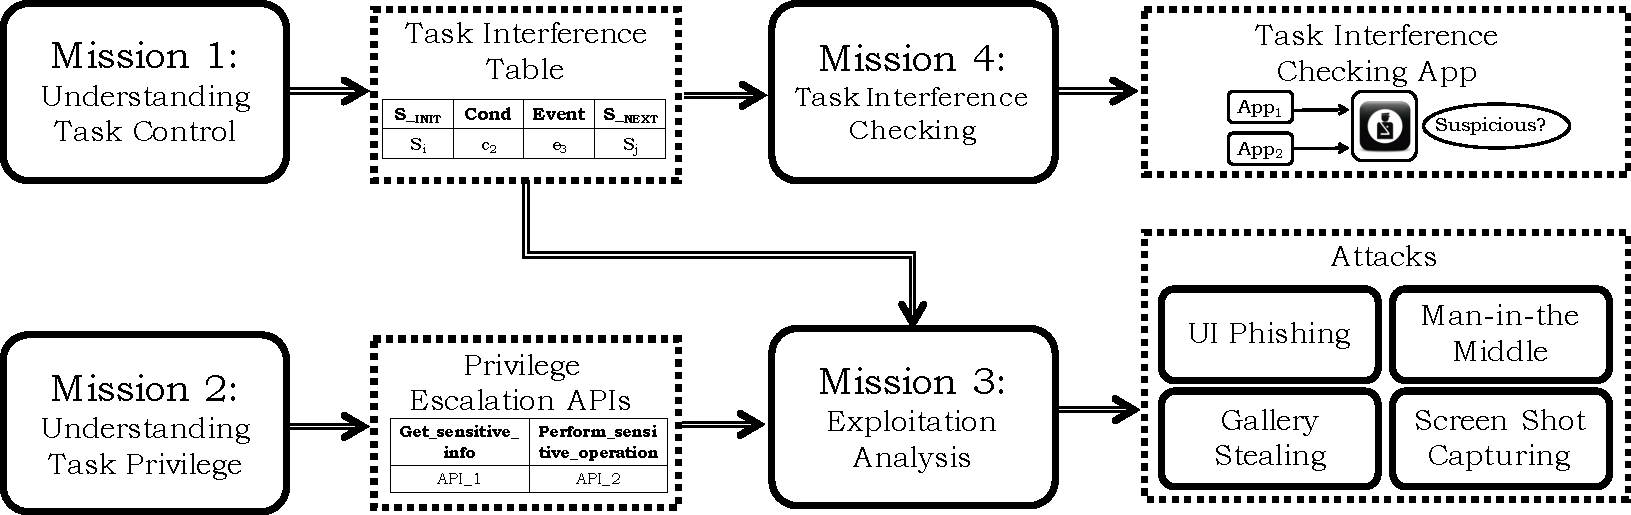
\includegraphics[width=1\linewidth]{overall.pdf}
        \caption{Approach Overview}
        \label{fig:arch}
\end{figure*}

\subsubsection{Approach Overview} \label{sec:approachoverview}

The goal of our work is to comprehensively analyze the Android task
mechanism to identify attacks, as well as creating solutions to
prevent such attacks.

As shown in Figure~\ref{fig:arch}, our research consists of four
components: \textsl{Understanding Task Control}, \textsl{Understanding
  Task Privilege}, \textsl{Exploitation Analysis} and \textsl{Task
  Interference Checking}.

The first component is to analyze the Android task mechanism,
identifying control conditions that can be leveraged by attackers.
We aim to find out the interference of tasks between two
apps, and identify the dominating factors deciding the apps'
property.  Secondly, we focus on studying the additional privilege
apps obtained when two apps are in the same task. We delicately test sensitive
system APIs and compare the difference of the results before and after
apps in the same task. Based on the understanding from the previous
stages, to demonstrate the achievability and severity of the
privilege escalation against Android task mechanism, we develop four light-weight
real-world attacks that can steal the sensitive information
successfully, most of which only requires \texttt{INTERNET}
permission.  At last, we design a task interference checking app to
detect the task interference between users' important apps and other
installed apps.

\subsection{Security Analysis of Android Task Structure}\label{sec:atmapproach}
In this subsection, we introduce our approach. We focus on two aspects of
the Android task mechanism. First, We analyze the conditions that
affect Android task control to identify different ways that can
include an app into a task. Second, we explore the privilege an app
can get when it is included into a task. These are two necessary
components to identify new attacks.


\subsubsection{Understanding Android Task Control Conditions}

We explore the conditions and actions of Android task control through
dynamic testing.  To do this, we examine the Android
documentation~\cite{taskdoc} to create test cases to drive the
exploration. Our goal is to check the influence of the flags
introduced in Section~\ref{sec:preliminaries} on the task mechanism.

{\noindent \bf Testing Methodology.} We implemented the two template
apps introduced in Section~\ref{sec:threatandapproach}, AppB and AppM, as the
inputs to drive the testing process.  For each combination of the
task-control-related flags, such as {\em launchMode} and {\em
  taskAffinity}, we set the corresponding value in app templates,
create a pair of AppB and AppM, and test them with different sequences
of launching events, e.g., using the Android Launcher to start AppB
(denoted as Launcher$\rightarrow$AppB) or using AppB to launch AppM
(denoted as AppB$\rightarrow$AppM). During our test, AppB's {\em
  taskAffinity} is set to ``TaskB''.  We only test the conditions
where AppM's {\em allowTaskReparenting} is set to ``true'', as a
``false'' value in this flag will not result in task interference.

The results are summarized in Table~\ref{tbl:taskinterference}.  We
are interested in cases with potential task interference, i.e., AppM
ends up running as part of TaskB.  We mark the cases for task
interference, i.e., AppM running as part of TaskB, with an asterisk
``*''. The cases without an asterisk attached are considered to be
safe. We list four identified dangerous cases below.

\begin{itemize}
  \item {\bf Case 2}. Under the conditions of this case, AppM is
    launched first by the Android Launcher, followed by AppB. Only
    AppM runs at the foreground, while AppB cannot be executed.

    In this case, AppM blocks AppB from execution, which is a case
    of denial-of-use to AppB.
  \item {\bf Case 4}. Under the conditions of this case, AppM is
    launched by the Android Launcher, followed by AppB. AppB runs in
    the foreground, and AppM runs in the background, both in TaskB.
  \item {\bf Case 9}. Under the conditions of this case, the Android
    Launcher starts AppM. AppM then starts AppB. AppB runs in
    the foreground, and AppM runs in the background, both in TaskB.
  \item {\bf Case 10}. Under the conditions of this case, the Android
    Launcher starts AppB. AppB then starts AppM. AppM runs in
    the foreground, and AppB runs in the background, both in TaskB.
\end{itemize}

Whether two Apps are in the same task can be determined by
viewing the \emph{Recents} screen which renders all processes that
were opened since last clearance\cite{recents}. \emph{Recents} screen
is rendered when a user presses the \emph{Recents} button which is
located at the third from left to right at the button bar followed by
\emph{Back} and \emph{Home} buttons. If two Apps are in the same task,
\emph{Recents} screen will only show one process other than two when
they do not reside in the same task. Note that according to our
experiment, flags such as \texttt{FLAG\_ACTIVITY\_CLEAR\_TOP} and
\texttt{FLAG\_ACTIVITY\_REORDER\_TO\_FRONT} do not pose a difference
than the \texttt{SIGLE\_TOP} in our case. Therefore, we only include
the \texttt{SINGLE\_TOP} flag in our Table~\ref{tbl:taskinterference}.

\begin{table*}
\scriptsize
\centering
\caption{Task Interference Table. We assume AppB is running with the
  task ``TaskB.'' In the events, the operation A$\rightarrow$B stands
  for A launches B. In the resulting state's status, F stands for
  execution in foreground; B stands for execution in background; X
  stands for not-running.}
\label{tbl:taskinterference}
\resizebox{\columnwidth}{!}{%
\begin{tabular}{|l|c|c|c|c|c|c|c|c|}
\hline
\textbf{Case \#}                              &
\multicolumn{4}{c|}{\textbf{Initial Conditions}}         &
\textbf{Events} &
\multicolumn{3}{c|}{\textbf{Resulting State}}           \\
\cline{2-5} \cline{7-9}
& AppB & \multicolumn{3}{c|}{AppM} & &
AppB &  \multicolumn{2}{c|}{AppM} \\
\cline{2-5} \cline{7-9}
& LaunchMode & LaunchMode & TaskAffinity & Reparenting &  & Status &
Status & Task\\
\hline \hline
1  &  standard or & standard or & TaskB  & True
   & Launcher$\rightarrow$AppB; Launcher$\rightarrow$AppM    & F & X & - \\

   &  singleTop or & singleTop or &        &
   &                                   &   &   &  \\

   & flag(SINGLE\_TOP) & flag(SINGLE\_TOP) & &
   &                                   &   &   &  \\
\hline
2  &  standard or & standard or & TaskB  & True
   & Launcher$\rightarrow$AppM; Launcher$\rightarrow$AppB    & X & F & TaskB \\

*  &  singleTop or & singleTop or &        &
   &                                   &   &   &  \\

   & flag(SINGLE\_TOP) & flag(SINGLE\_TOP) & &
   &                                   &   &   &  \\
\hline
3  &  singleTask or & standard or & TaskB  & True
   & Launcher$\rightarrow$AppB; Launcher$\rightarrow$AppM    & F & X & - \\

   & flag(NEW\_TASK) & singleTop or & &
   &                                   &   &   &  \\

   &                 & flag(SINGLE\_TOP) & &
   &                                   &   &   &  \\

\hline
4  &  singleTask or & standard or & TaskB  & True
   & Launcher$\rightarrow$AppM; Launcher$\rightarrow$AppB    & F & B & TaskB \\

*  & flag(NEW\_TASK) & singleTop or & &
   &                                   &   &   &  \\

   &                 & flag(SINGLE\_TOP) & &
   &                                   &   &   &  \\

\hline
5  &  singleTask or & singleTask or & TaskB  & True
   & Launcher$\rightarrow$AppB; Launcher$\rightarrow$ AppM     & B & F & TaskM \\

   & flag(NEW\_TASK) & flag(NEW\_TASK) & &
   &                                   &   &   &  \\
\hline

6  &  singleTask or & singleTask or & TaskB  & True
   & Launcher$\rightarrow$ AppM ; Launcher$\rightarrow$AppB    & F & B & TaskM \\

   & flag(NEW\_TASK) & flag(NEW\_TASK) & &
   &                                   &   &   &  \\
\hline

7  &  singleInstance or & any or & TaskB  & True
   & Launcher$\rightarrow$AppB; Launcher$\rightarrow$AppM    & F & X & - \\
\hline

8  &  singleInstance or & any or & TaskB  & True
   & Launcher$\rightarrow$AppM; Launcher$\rightarrow$AppB    & F & B & TaskM \\
\hline

9  &  standard or & standard or & TaskB  & True
   & Launcher$\rightarrow$AppM; AppM$\rightarrow$AppB  & F & B & TaskB \\

*   &  singleTop or & singleTop or &        &
   &                                   &   &   &  \\

   & flag(SINGLE\_TOP) & flag(SINGLE\_TOP) & &
   &                                   &   &   &  \\
\hline

10  &  standard or & standard or & TaskB  & True
   & Launcher$\rightarrow$AppB; AppB$\rightarrow$AppM  & B & F & TaskB \\

*   &  singleTop or & singleTop or &        &
   &                                   &   &   &  \\

   & flag(SINGLE\_TOP) & flag(SINGLE\_TOP) & &
   &                                   &   &   &  \\
\hline
\end{tabular}
}
\end{table*}

\subsubsection{Understanding Privilege Obtained in the Same Task}
\label{sec:priv}

From the results in Table~\ref{tbl:taskinterference}, we can see that
AppM has several ways to be included into the task of AppB, often
without involving actions from other apps or the system. Next, we
explore the privilege obtained through the Task mechanism, including
privilege for retrieving other apps' information and privilege for
changing other apps' states. Therefore, if the privilege given to apps
in the same task allows them to carry out dangerous actions, it can be
potentially misused by the malicious app.

\textbf{Retrieving Information of Other Apps}

\noindent

Figuring out the execution state of a victim app, such as whether it
is running and which activity is in foreground, is often used as the
first step in several attacks, such as UI
hijacking~\cite{UIstateinference}. Therefore, Android by default disallows one app
from directly querying another app's runtime information from through
the Android sandbox policy.

In older versions of Android, there were APIs allowing inter-app
runtime information checking.
For devices that are prior to \textit{Android Lollipop
  (v5.0)}, directly calling the API
\texttt{getRunningTasks(int maxNum)} will return the information of as
many as \texttt{maxNum} running activities~\cite{getrunningtask}.
However, this function is deprecated after \textit{Lollipop} since allowing third-party apps to invoke the function
directly will cause information leakage in important apps.

For devices prior to \textit{Android MarshMallow (v6.0)}, directly
calling \\
\texttt{getRunningAppProcesses()} returns a list of
application processes that are running on the
device~\cite{getrunningtask}. This function returns a
\textit{RunningAppProcessInfo} object, which includes a member
variable called \textit{importance} that represents the importance
level that the system places on the
process~\cite{processimportance}. It has one of these values:
\texttt{IMPORTANCE\_FOREGROUND}, \texttt{IMPORTANCE\_VISIBLE},
\texttt{IMPORTANCE\_SERVICE}, \texttt{IMPORTANCE\_BACKGROUND} and
\texttt{IMPORTANCE\_EMPTY}. If \textit{importance} is
\texttt{IMPORTANCE\_FOREGROUND}, the corresponding process is running
in the foreground. This method, however, cannot accurately point out
which activity running in the foreground since it operates on a
process level and accesses only the package name.  This method is also
no longer supported for \textit{MarshMallow} devices with API level 23
unless the third-party app who is making a call to this function has
the same process ID as the target process.


\paragraph*{Getting App Running Information in a Task.}
Although the Android API \\
\texttt{getRunningTasks()} is deprecated for
direct usage, we have found that it still works if the calling app and
the target app are in the same task.  The official documentation of
\texttt{getRunningTasks()} does not explicitly point it out but only
states that if it is called, this function only returns a small
subsets of information, e.g., the information of the caller's own task
and home task which is considered to be not
sensitive~\cite{getrunningtask}.


\textbf{Changing States of Other Apps}

\noindent

\paragraph*{UI Injection.}
Ideally, if an app is running in the foreground, other apps isolated
from this app should not perform sensitive operations on it. Chen {\em et
al.}~\cite{UIstateinference} show two UI-injection methods that do not
require any permissions: (1) starting an \texttt{Activity} by setting
\texttt{lauchMode=singleInstance}. This is also how most system apps,
such as the alarm app, pop up a window on the top of another
app~\cite{androidlaunchmode}; (2) starting an \texttt{Activity} from
the Android broadcast receiver~\cite{androidbroadcastreceiver}.

In our analysis, we find that if two apps are in the same task, the
UI-injection attack becomes easier.  The attacker can simply call the
function \texttt{startActivity()} to achieve the same effect. Through
understanding the Android SDK source code, \texttt{startActivity()}
invokes \texttt{startActivityForResult()} with
\texttt{requestCode=-1}. Later \\
\texttt{startActivityForResult()}
invokes \texttt{execStartActivity()} in the Instrumentation class, a
base class for implementing application instrumentation
code~\cite{Instrumentation}. \\
 \texttt{execStartActivity()} then checks
the base package of the calling activity by invoking
\texttt{getBasePackageName()}. If the base package of calling activity
matches with that of target activity, the Android system launches the
target activity.

\paragraph*{Terminating UI.}
Android does not allow a third-party app to terminate a running app
unless they are in the same process. Although an app is not in the
foreground, the Android system still allows any third-party apps to
make calls to
\texttt{killBackgroundProcesses()}~\cite{killBackgroundProcesses} to
terminate any specific background app. There is no direct way to
terminate a foreground-running activity.

Unlike \texttt{startActivity()}, even if two apps are in the same
task, calling \texttt{finish()} or \texttt{finishActivity()} will not
terminate the foreground activity, but will terminate the activity
that makes the call. However, we found that as long as two apps are in
the same task, calling the API \texttt{finishAndRemoveTask()} results
in terminating the whole Task regardless of whether an activity is
running in the foreground~\cite{finishAndRemoveTask} or not.
This provides the malicious app an interface to terminate other apps which are within the same task as it.

\subsection{Information Stealing Attacks}\label{sec:infoattack}
Based on analysis from Section~\ref{sec:atmapproach}, we develop
four proof-of-concept attacks: \textsl{UI Phishing},
\textsl{Activity-in-the-middle Attack}, \textsl{Gallery Stealing}, and
\textsl{Screen Shot Capture}. These four attacks demonstrate the
severity of the security problems we identified. In this subsection, the
attacks are illustrated using two most popular social apps, Instagram
and Facebook. Except Gallery Stealing, which requires
\texttt{READ\_EXTERNAL\_STORAGE}, all other three attacks only require
the \texttt{INTERNET} permission~(in order to send out the information
stolen).

\subsubsection{UI Phishing}
UI Phishing is a popular type of attacks to spoof users.  The
difficulty of phishing attack is to decide the timing when the
spoofing interface should be prompted, in order to prevent the victim
from noticing it.  Ren {\em et al.}~\cite{TaskHijacking} introduced
``Back Hijacking'', which directs users to a spoofed bank
\textit{LoginActivity}. The key difference is that the attack method
identified in our approach {\em actively} interact with the victim app
using the privilege obtained through the approaches we discussed in
Section~\ref{sec:priv}.

Our proof-of-concept UI Phishing attack is implemented against
the scenario when a user logs in to Instagram using his/her Facebook
account.  In order to ease understanding the phishing attack against
this scenario, we brief the Facebook SSO service.  According to the
Facebook Android developer documentation~\cite{FacebookLoginWays},
Facebook SDK takes three ways for apps who require Facebook Login as
part of functionality:

\begin{itemize}
\item {\bf Native App Login.}
If the Android device already has the Facebook app installed, pressing
the Facebook login button directly opens the Facebook app where user
can log in his/her Facebook account and grants permission to the
third-party app to access his/her Facebook personal information.

\item \textbf{Chrome Custom Tab Login. }
If the Android device does not have the Facebook app installed, a
third-party app can ask the Chrome browser to open Facebook login page
by registering a scheme in the \texttt{Manifest} with the format
\texttt{fb+facebook\_app\_id}.

\item {\bf WebView Login.}
Finally if neither the Android device has Facebook app installed, nor
does the third-party app register for Chrome Custom Tab Login, an
embedded WebView will be launched dynamically rendering the content of
Facebook login page.
\end{itemize}

Our attack works when a user presses the ``Log in with Facebook''
button in Instagram. We assume that a user already has Facebook App
installed in the device. Instagram includes Facebook Login as a part
of its functionality. It does not register for Chrome Custom Tab
Login. In other words, after pressing the ``Log in with Facebook''
button in Instagram, it will launch Facebook App directly. The package
name of Facebook app is \texttt{"com.facebook.katana"}, the package
name of self-build WebView is \texttt{"com.android.webview"} and the
package name of Instagram is \\
\texttt{"com.instagram.android"}.  Shown
in Figure~\ref{fig:uiphishing}, it works in the following steps.

\begin{figure*}[t!]
        \centering
        \begin{subfigure}[t]{0.5\textwidth}
                \centering
                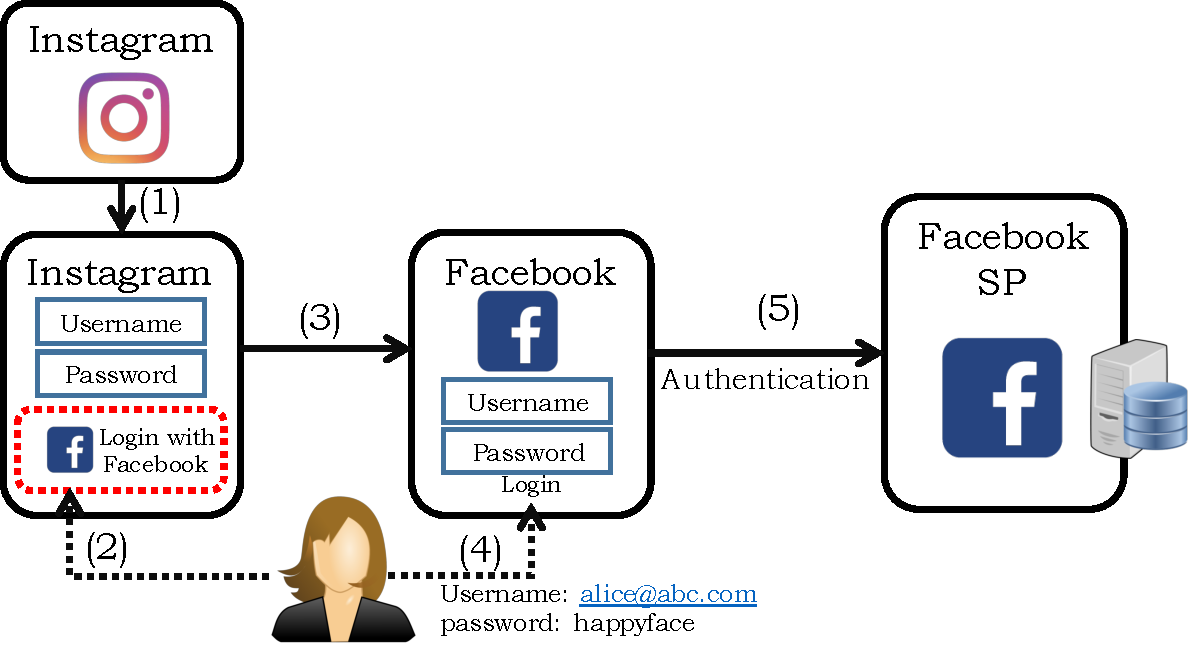
\includegraphics[width=\linewidth]{attack-phishing-0.pdf}
                \caption{Single-Sign-On Architecture}
          \end{subfigure}%
          %\quad
        \begin{subfigure}[t]{0.5\textwidth}
                \centering
                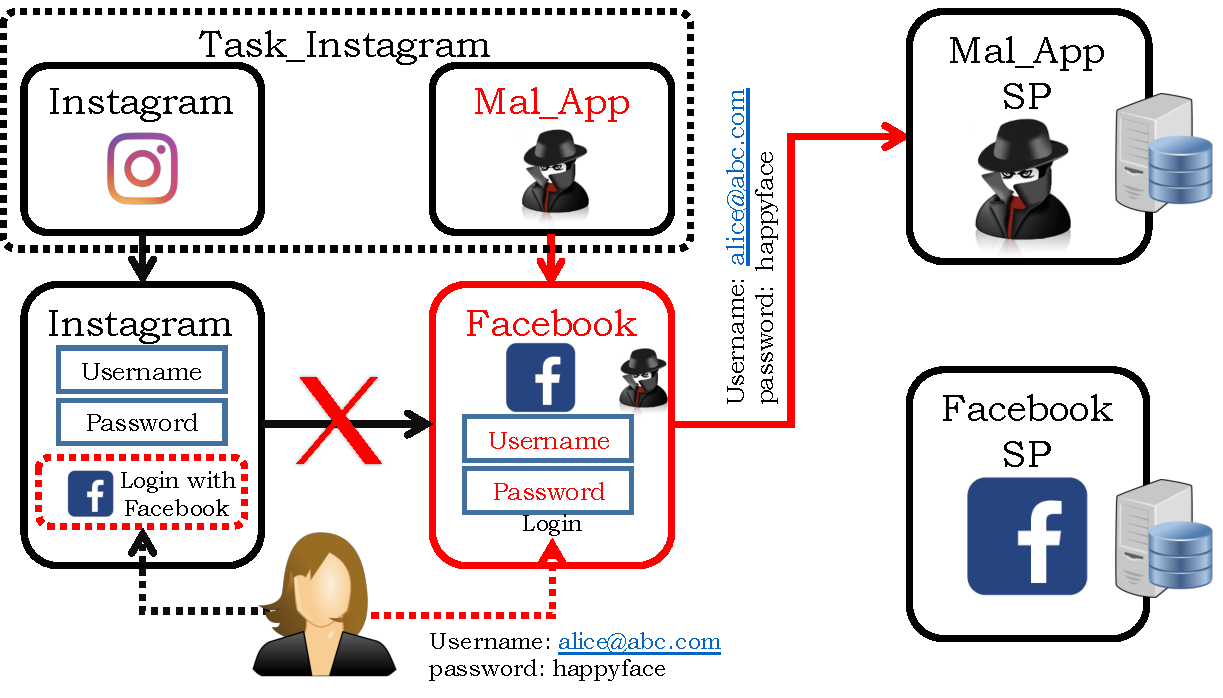
\includegraphics[width=\linewidth]{attack-phishing-1.pdf}
                \caption{UI Phishing Attack}
        \end{subfigure}
        \caption{UI Phishing.}
         \floatfoot{(a) When the user selects
          ''login with Facebook'' in Instagram, Instagram will launch
          the Facebook app. After the user inputs username, password
          and finishes the authentication with the Facebook service
          provider, Instagram gets the permission to access the user's
          Facebook resources. (b) The malicious app Mal\_App declares
          same taskAffinity as Instagram. Mal\_App creates a
          background thread and monitors the running states of
          Instagram. When the user selects Facebook login button and
          Instagram launches the Facebook activity, Mal\_App will
          override Facebook with a fake login UI. The
          username/password input by the user will be sent to
          Mal\_App's service provider.}
           \label{fig:uiphishing}
\end{figure*}



\textbf{(1)} Attacking app declares the same task as Instagram. This step
can be achieved by setting the attributes of \textit{taskAffinity} and
\textit{allowTaskReparenting} as follows.
\begin{lstlisting}[language=XML]
 <activity
            android:name=".UIPhishingActivity"
            android:allowTaskReparenting="true"
            android:taskAffinity="com.instagram.android">
\end{lstlisting}

\textbf{(2)} The launcher first launches the attacking app, which
launches Instagram immediately through invoking the task parent since
Instagram is the parent of the current task. Before Instagram's
\texttt{setContentView(R.layout.main)} function can be called, the
attacking app launches Launcher (Home), meaning that Instagram cannot
be displayed in order to achieve the stealthiness. The process can be completed in a fairly short time and will not be noticed by the victim with bare eyes. After that, our attacking app waits for victim to launch Instagram herself.


\textbf{(3)} The attacking app then creates a background thread which
runs in a cycle of, we devise, every 100 milliseconds. In the
meantime, it checks whether there is a change in the foreground
package name, i.e., in our case, the package name changes from \\
\texttt{"com.android.webview"} to \texttt{"com.facebook.katana"}. This
can be achieved by simply making API call to
\texttt{getRunningTasks()}. Once the foreground package has been
changed to Facebook, our attack pops up our counterfeit Facebook
\textit{LoginActivity} overriding the real one. The spoofed UI
collects the user's login information and send it to adversary's
back-end server.

\subsubsection{Activity-in-the-middle Attack}
The Facebook SSO process is based on OAuth
2.0~\cite{OAuthDemystified}. The main steps of this mechanism are: (1)
When the user opens the relying party (RP) app, in our case,
Instagram, it passes its \texttt{Facebook\_app\_id} and directed URL
to the Android System.  (2) The Android system then redirects user to
the Service Provider (SP), in our case, Facebook, and passes it the
\texttt{Facebook\_app\_id}.  (3) If the user requests to grant the
permission to the RP, SP will issue an access token to the Android
system.  (4) The Android system passes the access token to RP, by
which RP is able to access the user's protected resource on SP.

Facebook has two types of access tokens, short-term and
long-term~\cite{fbaccesstoken}. Short-term access token lasts several
hours and long-term lasts for 60 days. Unless specifically required,
Facebook usually issues short-term access token. RPs use graph API
provided by Facebook to retrieve protected resources hosted on
Facebook server~\cite{graphapi}. Graph API is an HTTP-based API, which
is implemented as the following URL:
 \begin{lstlisting}
 https://graph.facebook.com/me?fields=xxx&access_token=xxx
 \end{lstlisting}

In other words, any party who has the access token can access the
user's protected resources hosted on Facebook servers.

In Android, redirecting to the Facebook app is done by intent
transition based on \texttt{startActivityForResult()} and
\texttt{onActivityResult()}.  We implement an MITM attacking app whose
model runs in the following steps, shown in Figure~\ref{fig:mitm}.

\textbf{(1)} It follows the first three steps in the UI Phishing
attack model.

\textbf{(2)} Instead of popping up a phishing login
page like UI Phishing, the MITM attack pops up a transparent activity,
which blocks the traffic that is supposed to be relayed to Facebook
server from user's device system and passes our own traffic to
Facebook. This step can be easily realized by creating an invisible
Facebook Login Button and sending a button pressed event itself by
invoking \texttt{mFacebookLoginBtn.performClick()}.

\textbf{(3)} After the user grants the permission, which he/she
intends for Instagram, the MITM app retrieves the access token. Since
Instagram runs in the background, once the foreground finishes,
Instagram will be invoked.


\textbf{(4)} To finalize the process, the adversary needs to verify
\texttt{APP\_ID} and \emph{App Secret} with Facebook. An adversary can
either register its attacking app in Facebook Developer Website and
use its own \texttt{APP\_ID} and \emph{App Secret} or steal other RP
apps' ID and Secret. Facebook RP Apps will post an HTTP message when
user system launches native Facebook App.

\begin{figure*}[t]
        \centering
        \begin{subfigure}[t]{0.5\textwidth}
                \centering
                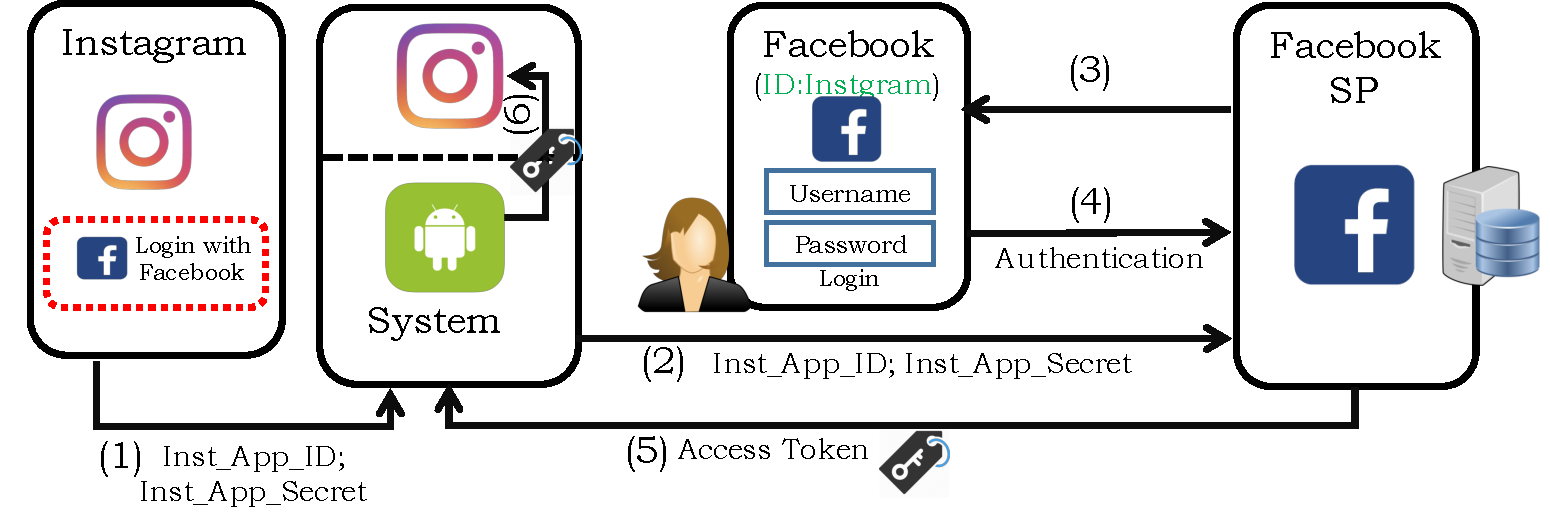
\includegraphics[width=\linewidth]{attack-mim-0.pdf}
                \caption{Single-Sign-On Permission Granting Architecture}
          \end{subfigure}%
          %\quad
       \begin{subfigure}[t]{0.5\textwidth}
                \centering
                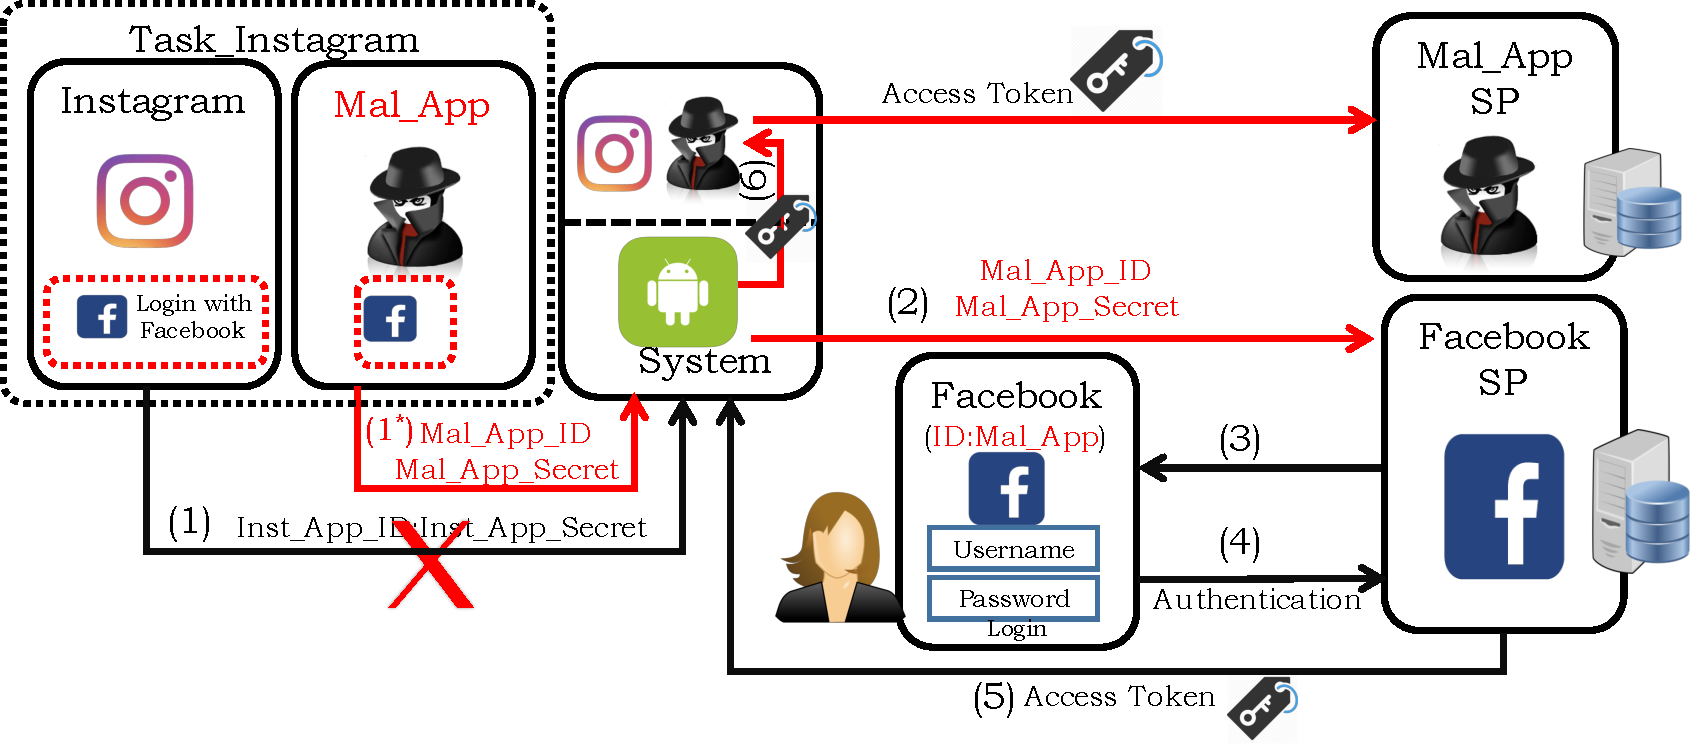
\includegraphics[width=\linewidth]{attack-mim-1.pdf}
                \caption{Activity-in-the-Middle Attack}
        \end{subfigure}
        \caption{Activity-in-the Middle Attack on SSO.}
        \floatfoot{(a) When a
          user wants to login with Facebook in the Instagram,
          Instagram sends system its application ID with application
          secret, Inst\_App\_ID and Inst\_App\_Secret. Android system
          forwards request with Inst\_App\_ID and Inst\_App\_Secret to
          Facebook service provider and retrieves Facebook Login
          Activity bound with Inst\_App\_ID. The user inputs her/his
          username/password for authentication. Facebook service
          provider returns the access token to Android system if the
          authentication passed. Android system sends the access token
        to Instagram according to the application ID that system
        received. (b) The malicious app Mal\_App overrides the
        ownership of the Instagram task in the same way as
        UI-phishing. It monitors the Instagram running status and
        sends system its Facebook login request (including Mal\_App\_ID and
        Mal\_App\_Secret) before the Instagram's request arrives
        Android system. Android system sends Mal\_App's request to
        Facebook service provider and
        drops the same login request arrived later. Facebook return
        Login Activity bound with Mal\_App\_ID. The user inputs her/his
          username/password for authentication. Facebook service
          provider returns the access token to Android system if the
          authentication passed. Android system sends the access token
        to  Mal\_App according to the application ID that system
        received.}
        \vspace{-0.2cm}
           \label{fig:mitm}
\end{figure*}

\subsubsection{Gallery Stealing}
Starting from Android 6.0 (API level 23), in order to access gallery,
an app has to request for \texttt{READ\_EXTERNAL\_STORAGE} permission
at runtime rather than at the installation time, which is classified
as one of the dangerous permissions~\cite{permissionruntime}. This
mechanism provides more secure and flexible protection to user's photo
gallery.  However, this new security mechanism can be bypassed by
exploits to the Android task mechanism, as shown in this subsection.

\noindent\textbf{Timing.} 
For Android devices before \textit{marshmallow} (API level lower than
23), permissions are requested at the time when an app is being
installed. Apps with suspicious permissions will easily trigger the
user's attention and likely be denied access. However, with the new
requesting-permissions-at-run-time mechanism, our attacking app can
avoid requesting permission when being installed since it is requested
at the run time. To figure out the suitable timing, it continuously
monitors Instagram.  Once the victim clicks the ``Camera'' button on
Instagram which allows Instagram to access the gallery and camera, our
attacking app instantly kills Instagram and pops up our requesting
dialog for access photos in gallery. User mistakenly believes that
he/she is granting the permission to Instagram. After the permission
is granted, our attacking app retrieves all the photos from user's
gallery and send them to the back-end server. In order to be
stealthier, the attacking app pops up a dialog shows ``System
encounters errors'' and finally kills itself.

\noindent\textbf{Permission Dialog.}
Even though timing improves the naturalness of the attack, Android
permission dialog shows the name of the app in bold who makes the
request. We propose two ways to circumvent this
problem.
\\\textbf{(1)} By employing the idea of social engineering, the attacker can name the attacking app 
using a name similar to the target app. In our case,
e.g., ``Instgram'' or ``Instagam''. However, naming the app in this way
can hardly pass the review of Google Play. Even if it does, careful
users may still notice the difference. Therefore, in our attack, we do not
use this method.

\noindent \textbf{(2)} Employing the tapjacking. The idea of tapjacking
is putting message the attacker wishes to display on the top of the
real system message by setting a window layout flag
\texttt{TYPE\_SYSTEM\_OVERLAY}. Android realizes the potential threat
and adopts the mechanism
\texttt{MotionEvent.FLAG\_WINDOW\_IS\_OBSCURED} which alerts the real
dialog is being overlaid\cite{flagwindowobscured}. Unfortunately,
Bana\'s\cite{TapjackingIwo} found that \\
\texttt{MotionEvent.FLAG\_WINDOW\_IS\_OBSCURED} is not triggered if
the covered text does not cover the touch points, which are the
buttons in the dialog. Android does not give a patch to the issue.
Instead, it adopts an intent transition scheme to notify the user that
the content is being overlaid starting from Android 6.0 (API level
23). We managed to circumvent the issue by implementing our main
attacking app with \texttt{targetSdkVersion=23}, and in the target app
we tricked the user to install a helper package, which is an
activityless service.  Only app which has the
\texttt{targetSdkVersion=22} and has the overlaying functionality
implemented. It seems tricking users to install additional package is
not applicable, but it is in fact a very common situation for many
apps such as those who require Android SQLite Manager.

The basic steps of the attack model are listed as
follows.

\textbf{(1)} The attack follows the first three steps of UI Phishing
attack.

\textbf{(2)} Once a user presses the camera button of Instagram as
shown in Figure~\ref{fig:gallery}(a), the foreground \texttt{Activity}
will change to
\texttt{"com.instagram.android.creation.activity.\-MediaCaptureActivity"}. Therefore,
Instead of detecting whether the foreground package has changed to
another app, we zoom in the design to focus on changing of the
foreground \texttt{Activity}.

\textbf{(3)} Instead of popping up a counterfeit
page like UI Phishing does, it pops up an \texttt{Activity} which
immediately asks a user for \texttt{READ\_EXTERNAL\_STORAGE} so that
the user thinks he/she is granting the permission to Instagram.

\textbf{(4)} Once the attack app gets the permission, it traverses all the pictures and transmits the image buffers to server.

\textbf{(5)} To achieve better stealthiness, we introduce the
Tapjacking to assist our attack. Its basic idea is to cover the real
texts with some fake texts. Then we are able to change the text of the
permission dialog to ``Allow Instagram to access ...?'' instead of the
real text which is ``Allow GalleryStealing to access ...?'', which is
shown in Figure~\ref{fig:gallery}(b). Once user grants the
permission, the app quickly sends all images as buffer to the server.
Meanwhile, it fools the user by showing a ``system warning dialog''
telling the user that the system encounters an error (shown in
Figure~\ref{fig:gallery}(c)).


\begin{figure*}[t]
        \centering
        \begin{subfigure}[b]{0.325\textwidth}
                \centering
               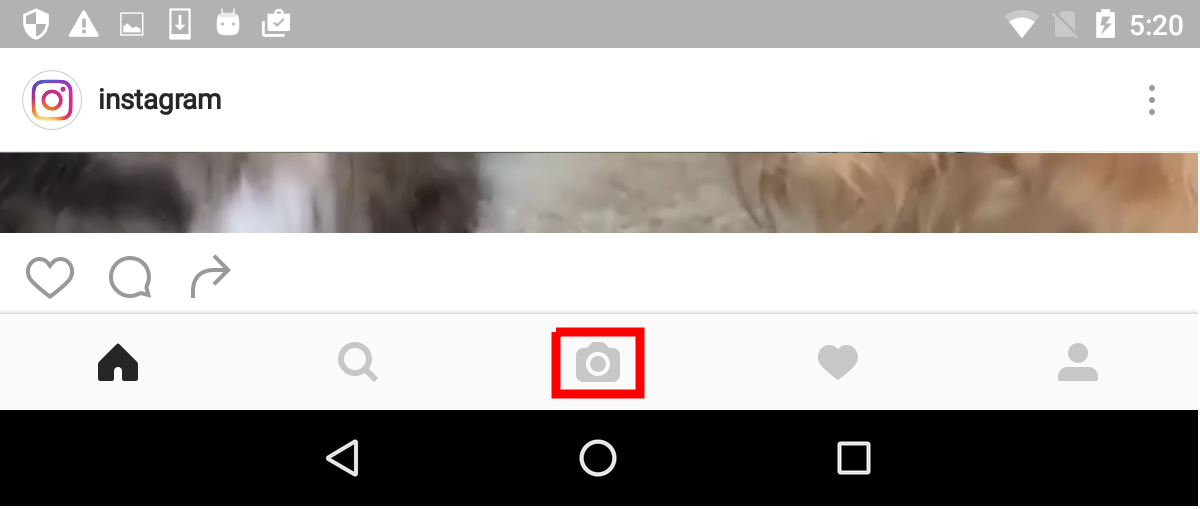
\includegraphics[width=\linewidth]{4-1}
                \caption{}
        \end{subfigure}
        \begin{subfigure}[b]{0.3\textwidth}
                \centering
          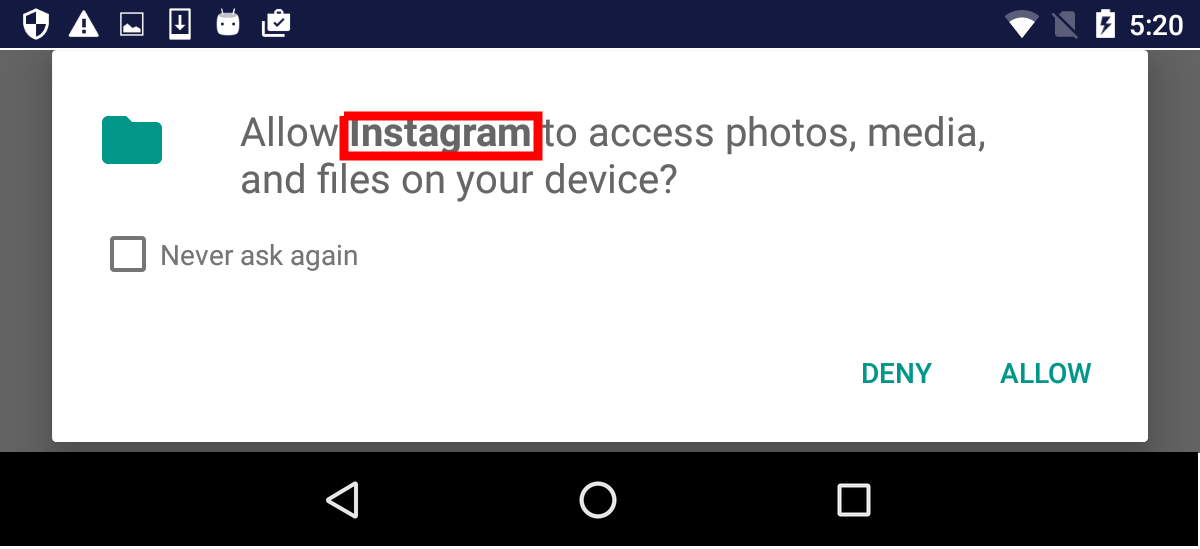
\includegraphics[width=\linewidth]{4-2}
                \caption{}
        \end{subfigure}
        \begin{subfigure}[b]{0.35\textwidth}
                \centering
          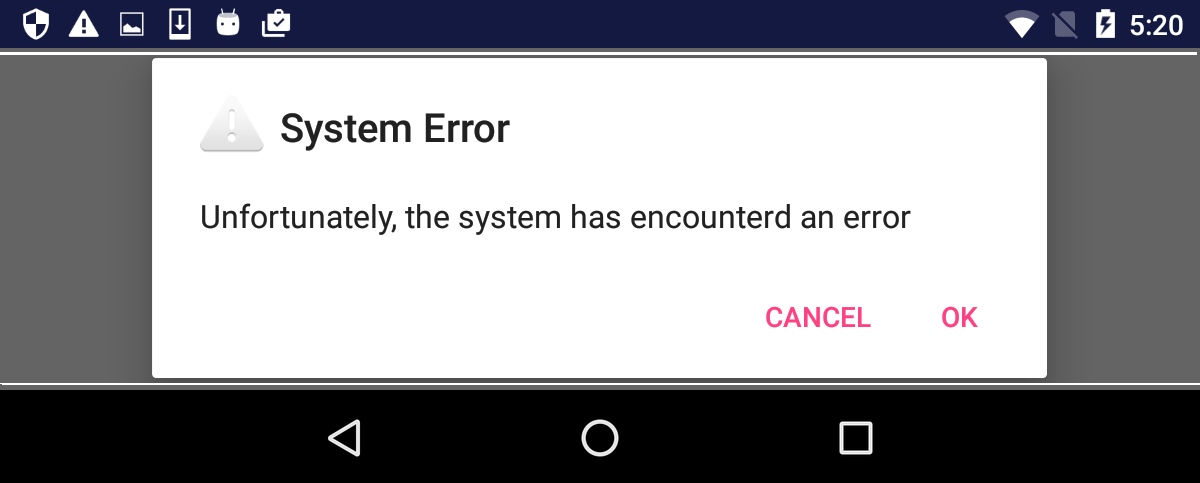
\includegraphics[width=\linewidth]{4-3}
                \caption{}
        \end{subfigure}
         \caption{Gallery Stealing Attack.}
         \floatfoot{First the user clicks the camera button highlighted in the first picture. Then the attacking app	kills the real Instagram and pops up its \texttt{Activity} asking for user permission, the text of permission dialog is overlaid by the fake text as shown in the second picture. Once user grants the permission, the app quickly sends all images as buffer to the server, meanwhile, it fools the user by showing a ``system'' warning dialog telling the user the system encounter an error.}
         \label{fig:gallery}
\end{figure*}

\subsubsection{Screen Shot Capturing}
With the ability of knowing which \texttt{Activity} is currently
running in the foreground, we implement this screen shot capturing
attack which starts taking screen shots while a user is entering
username and password in the Facebook \texttt{LoginActivity} which is
\texttt{com.facebook.katana.LoginActivity} in full. For password
typing, every time a character is entered, the character will be shown
for a short time before it turns into a star sign. Therefore, taking
screen shot every 0.1 second should capture everything a user types in
password box.


With respect to taking a screen shot programmatically, we summarize
four possible ways:
\begin{itemize}
\item {\bf Using READ\_FRAME\_BUFFER Permission.}  Declaring
  \texttt{READ\_FRAME\_BUFFER} permission in the \texttt{Manifest}
  allows an application to take screen shots by making calls to
  \texttt{ISurfaceComposer} \cite{framebuffer}. However, this
  permission is not available to third-party application unless it has
  the same signature as the system does.

\item {\bf Using fb*.} Some Linux systems store frame buffers in
  \texttt{/dev/graphics/fb*} or \texttt{/dev/fb*}. \texttt{fb0}
  represents the first frame buffer, \texttt{fb1} represents the
  second frame buffer and so on.  Using native C/C++ code to get
  access to these files and copy the buffer as a \texttt{GGLSurface}
  structure is theoretically possible. But there are two unsolvable
  obstacles of this method:
  \begin{itemize}
  \item This method requires root permission.
  \item It is likely that \texttt{fb*} does not even exist.
  \end{itemize}

\item {\bf Using Backup Channel over USB.}  Android system uses
  Android Debug Bridge (ADB) to listen to the debugging connections
  over USB~\cite{adb}. ADB has slightly more privileges than normal
  apps. Bai {\em et al.}~\cite{DBLP:conf/iceccs/BaiSWYLDG15} manage to
  exploit Backup Channel through ADB to steal access tokens from other
  apps. Combining ADB with Dalvik Debug Monitor Server (DDMS) tool
  enables an app to get the screen shot from the device without any
  permission~\cite{ddms}.

\item {\bf Using MediaProjection.}  For devices beginning in Android
  5.0 (API level 21), a class called \texttt{MediaProjection} was
  added to Android SDK which enables a third-party app to capture
  screen shot and record system audio\cite{mediaprojection}. While
  recording system audio requires \texttt{RECORD\_AUDIO} permission,
  capturing screen shots does not.
\end{itemize}

We employed the fourth method to capture screen shots. The basic steps
of the attack are listed as follows.\\ \textbf{(1)} It follows the
first three steps of UI Phishing. What's different is we devise this
attack to focus on Facebook App since we are hoping to steal user's
Facebook username and password. Hence, we declared this attack to
reside in the same task as Facebook.\\ \textbf{(2)} Once a user launches
the Facebook app, a transparent Activity is popped up start taking
screenshots. Although it does not require permission for taking screen
shots, it uses intent transition to let the user decide whether or not
an app can capture screen shots in a permission-like dialog. Again we
employ the tapjacking in Gallery Stealing attack to cover the text to
be ``Allow Facebook start accessing Internet?'' \\ \textbf{(3)} The
attack starts capturing screens by calling
\texttt{startActivityForResult()} which passes a screenshot as an
intent from which we can extract an object of \texttt{MediaProjection}
later, and finally use this \texttt{MediaProjection} object to pass
the image to an object of \texttt{ImageReader} through its member
function \texttt{createVirtualDisplay}. Since the screenshots are
taken in the \texttt{RGBA\_8888} format while bitmap takes
\texttt{ARGB\_8888}, we still need to do matrix transformations to
get the image.

\begin{figure*}[t]
        \centering
        \begin{subfigure}[b]{0.285\textwidth}
                \centering
               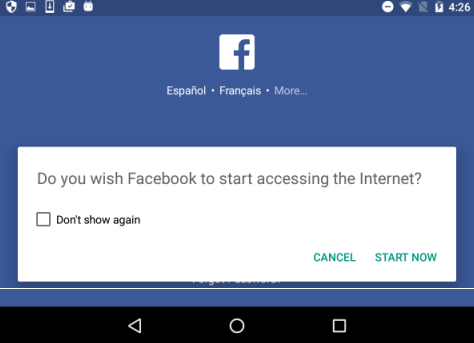
\includegraphics[width=\linewidth]{5-1}
                \caption{}
        \end{subfigure}
        \begin{subfigure}[b]{0.35\textwidth}
                \centering
          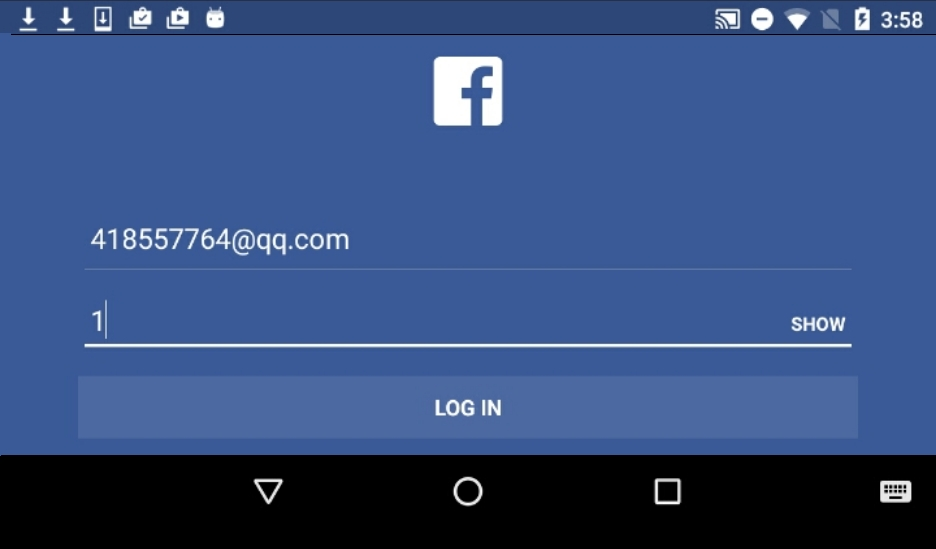
\includegraphics[width=\linewidth]{5-2}
                \caption{}
        \end{subfigure}
        \begin{subfigure}[b]{0.31\textwidth}
                \centering
          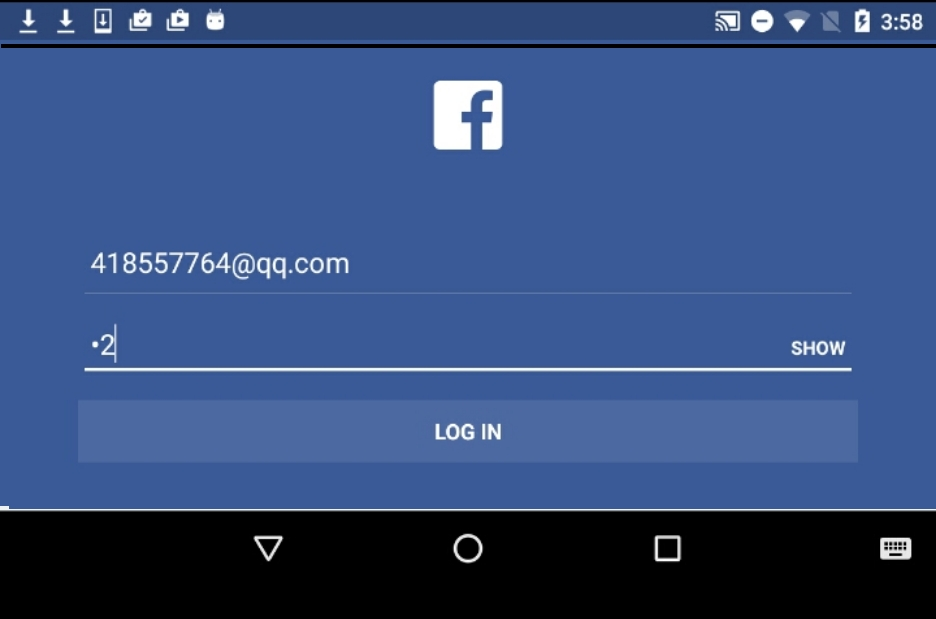
\includegraphics[width=\linewidth]{5-3}
                \caption{}
        \end{subfigure}
         \caption{Screenshot Capturing Attack.}
         \floatfoot{First the user launches Facebook, then the attacking app launches a transparent \texttt{Activity} which quickly asks for taking screen shot, the notification dialog is again overlaid by fake text as shown in the first picture. Once the user clicks start now, the attacking app begins to take screen shots as well as sending the screen shots to back end server. (b) and (c) are two of the screen shots received by server which expose the password plaintext.}
         \vspace{-0.2cm}
         \label{fig:memory}
\end{figure*}

\subsection{Attack Performance}\label{sec:attackperf}

In order to study the feasibility of the four attacks, we implement them and evaluate them in
two aspects, \emph{time cost} and \emph{memory usage}.
% We check the average running time and the average virtual memory curves to illustrate the performance of our four proof-of-concept attacks.

\subsubsection{Time Cost}
We conduct 6 - 8 rounds of tests for every attack to calculate the average
running time cost. The testing results are summarized
in Table~\ref{tbl:time}. As shown in Table~\ref{tbl:time}, our attacks
are efficient since the time cost of most attacks is less than 8 seconds:
the UI Phishing attack costs 7.1 seconds, which includes user
interactions such as launching Instagram, entering username and
passwords; The Activity-in-the-middle attack costs time 5.8 seconds; and
the average time cost of the gallery-stealing attack is 4.6 seconds.

The Screenshot Capturing attack is an exception, taking 38.1
seconds. This attack uses much longer time because screenshots in
Android are passed in the format of RGBA, while we need to change to
ARGB in order to convert it to common format such as JPEG and PNG.
We perform the matrix transformation required for the conversion on
the mobile device. But since the process is undertaken in the background, it will
not trigger the suspicions of the user. In the real world attack, an
adversary can leave the job of matrices transformation to the server.

\begin{table}[h]
  \centering
\caption{Time Cost of Proof-of-Concept Attacks}
\label{tbl:time}
\begin{footnotesize}
\begin{tabular}{|c|c|}
  \hline
  \textbf{Attack} & \textbf{Time Cost (s)} \\
  \hline\hline
  UI Phishing & 7.1\\
  \hline
  Activity-in-the-Middle & 5.8\\
  \hline
  Gallery Stealing & 4.6 \\
  \hline
  Screenshot Capturing & 38.1\\
  \hline
\end{tabular}
\end{footnotesize}
\end{table}

\subsubsection{Memory Usage}

We conduct 3-round experiments for each attacks to get the memory
distractions of attacks and evaluate their average memory usage. The
testing results are illustrated in Figure~\ref{fig:memory}.  It shows
that the maximum memory usage of most attacks is less than $70MB$ except
Gallery Stealing attack, whose memory usage is around $100MB$. Our
testing results also disclose the memory usage distribution on
different period, in which the major memory usage of each attack is to
launch victim app (normal app), e.g., Instagram and Facebook. The
memory usage differences caused by stealthy behaviors/operations are
negligible.

\begin{figure}[h]
        \centering
        \begin{subfigure}[t]{0.5\textwidth}
                \centering
               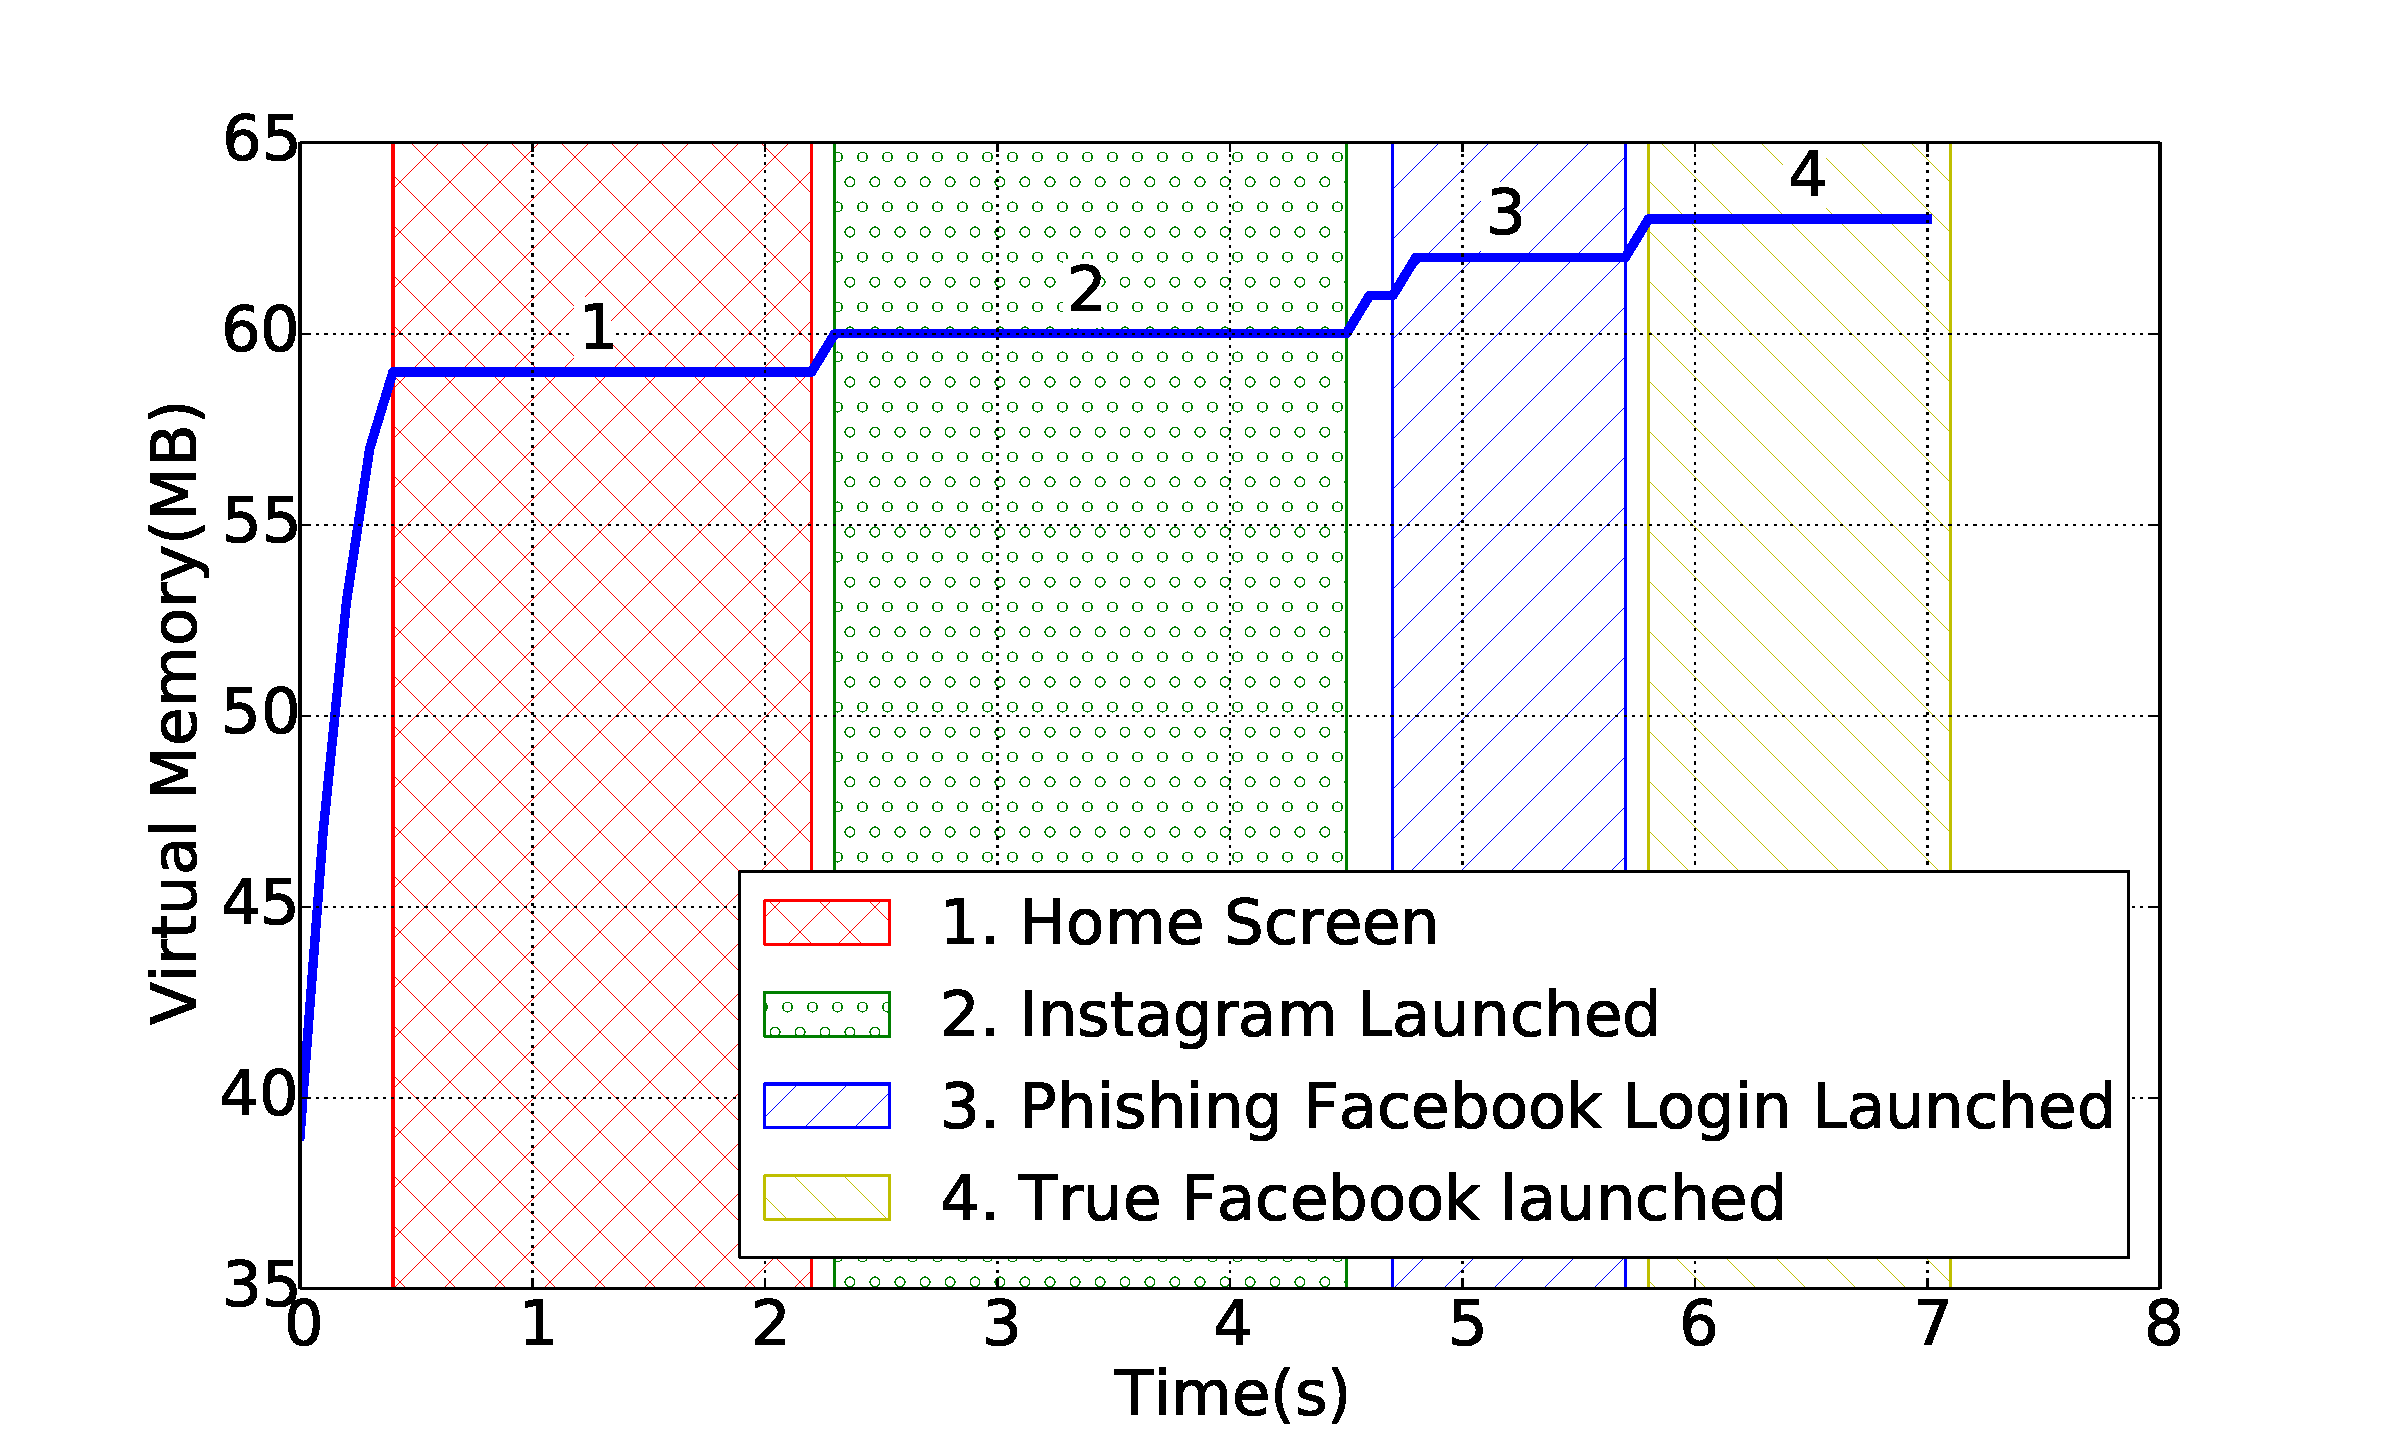
\includegraphics[width=\linewidth]{attack1memory.pdf}
                \caption{UI Phishing}
        \end{subfigure}%
        %\quad
        \begin{subfigure}[t]{0.5\textwidth}
                \centering
          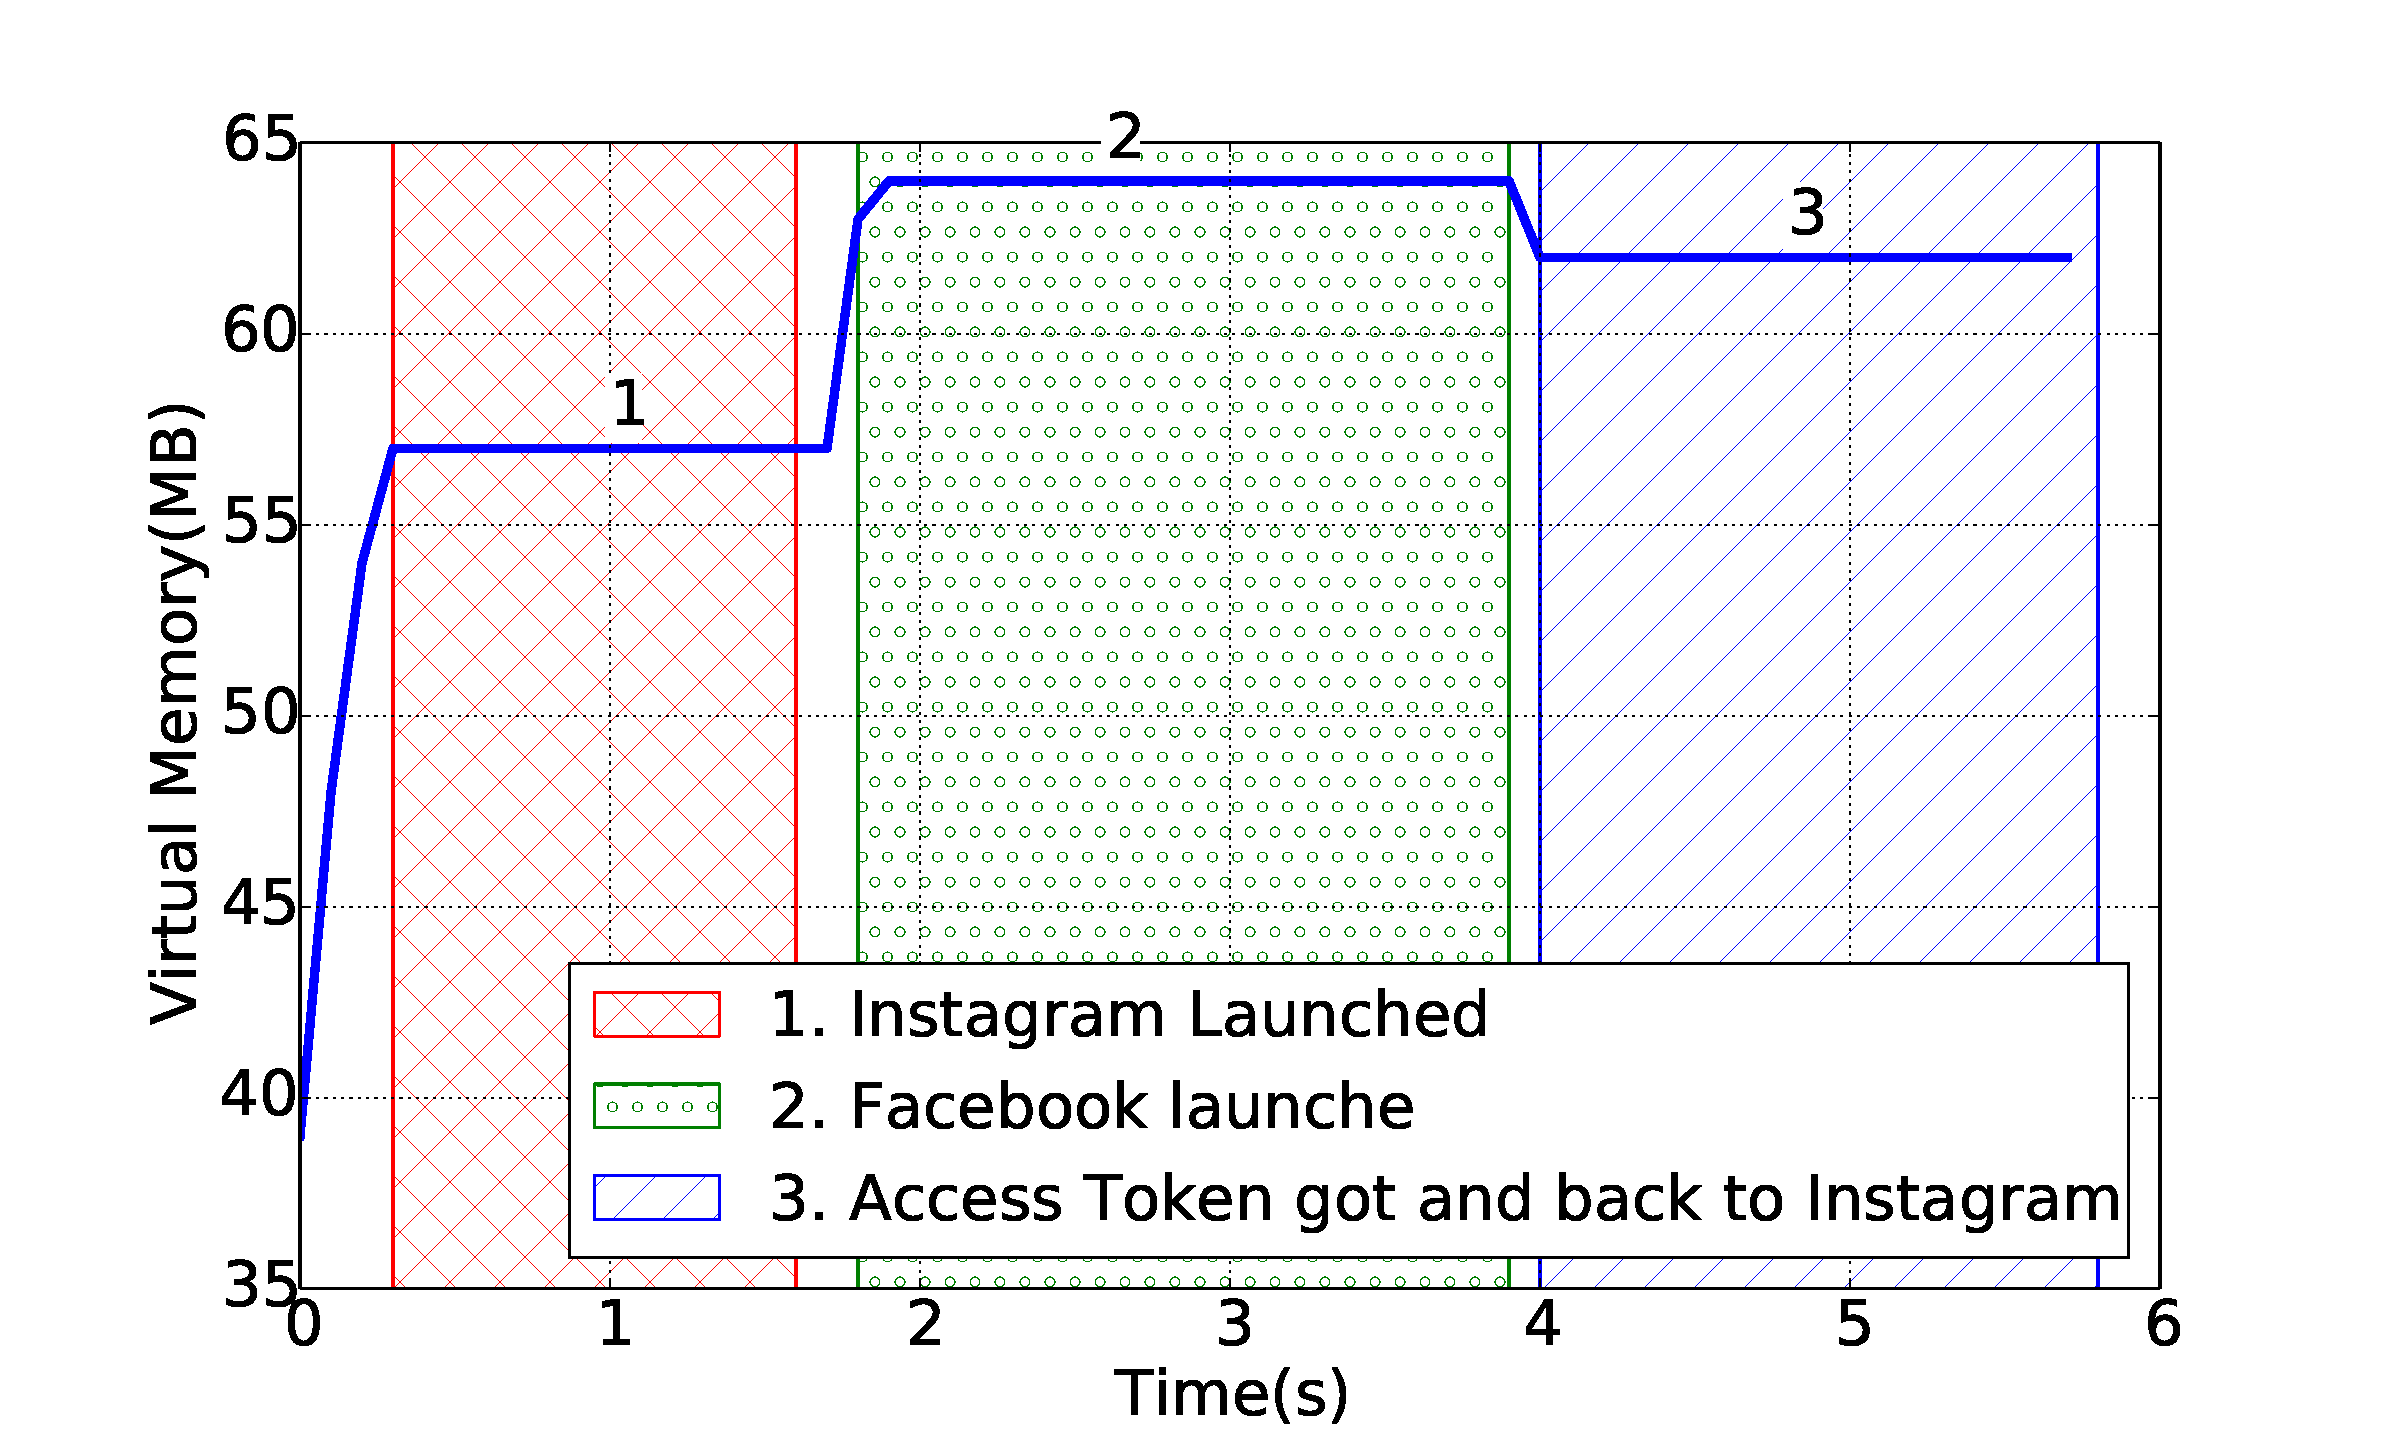
\includegraphics[width=\linewidth]{attack2memory.pdf}
                \caption{Activity-in-the-middle}
        \end{subfigure}
        \begin{subfigure}[t]{0.5\textwidth}
                \centering
          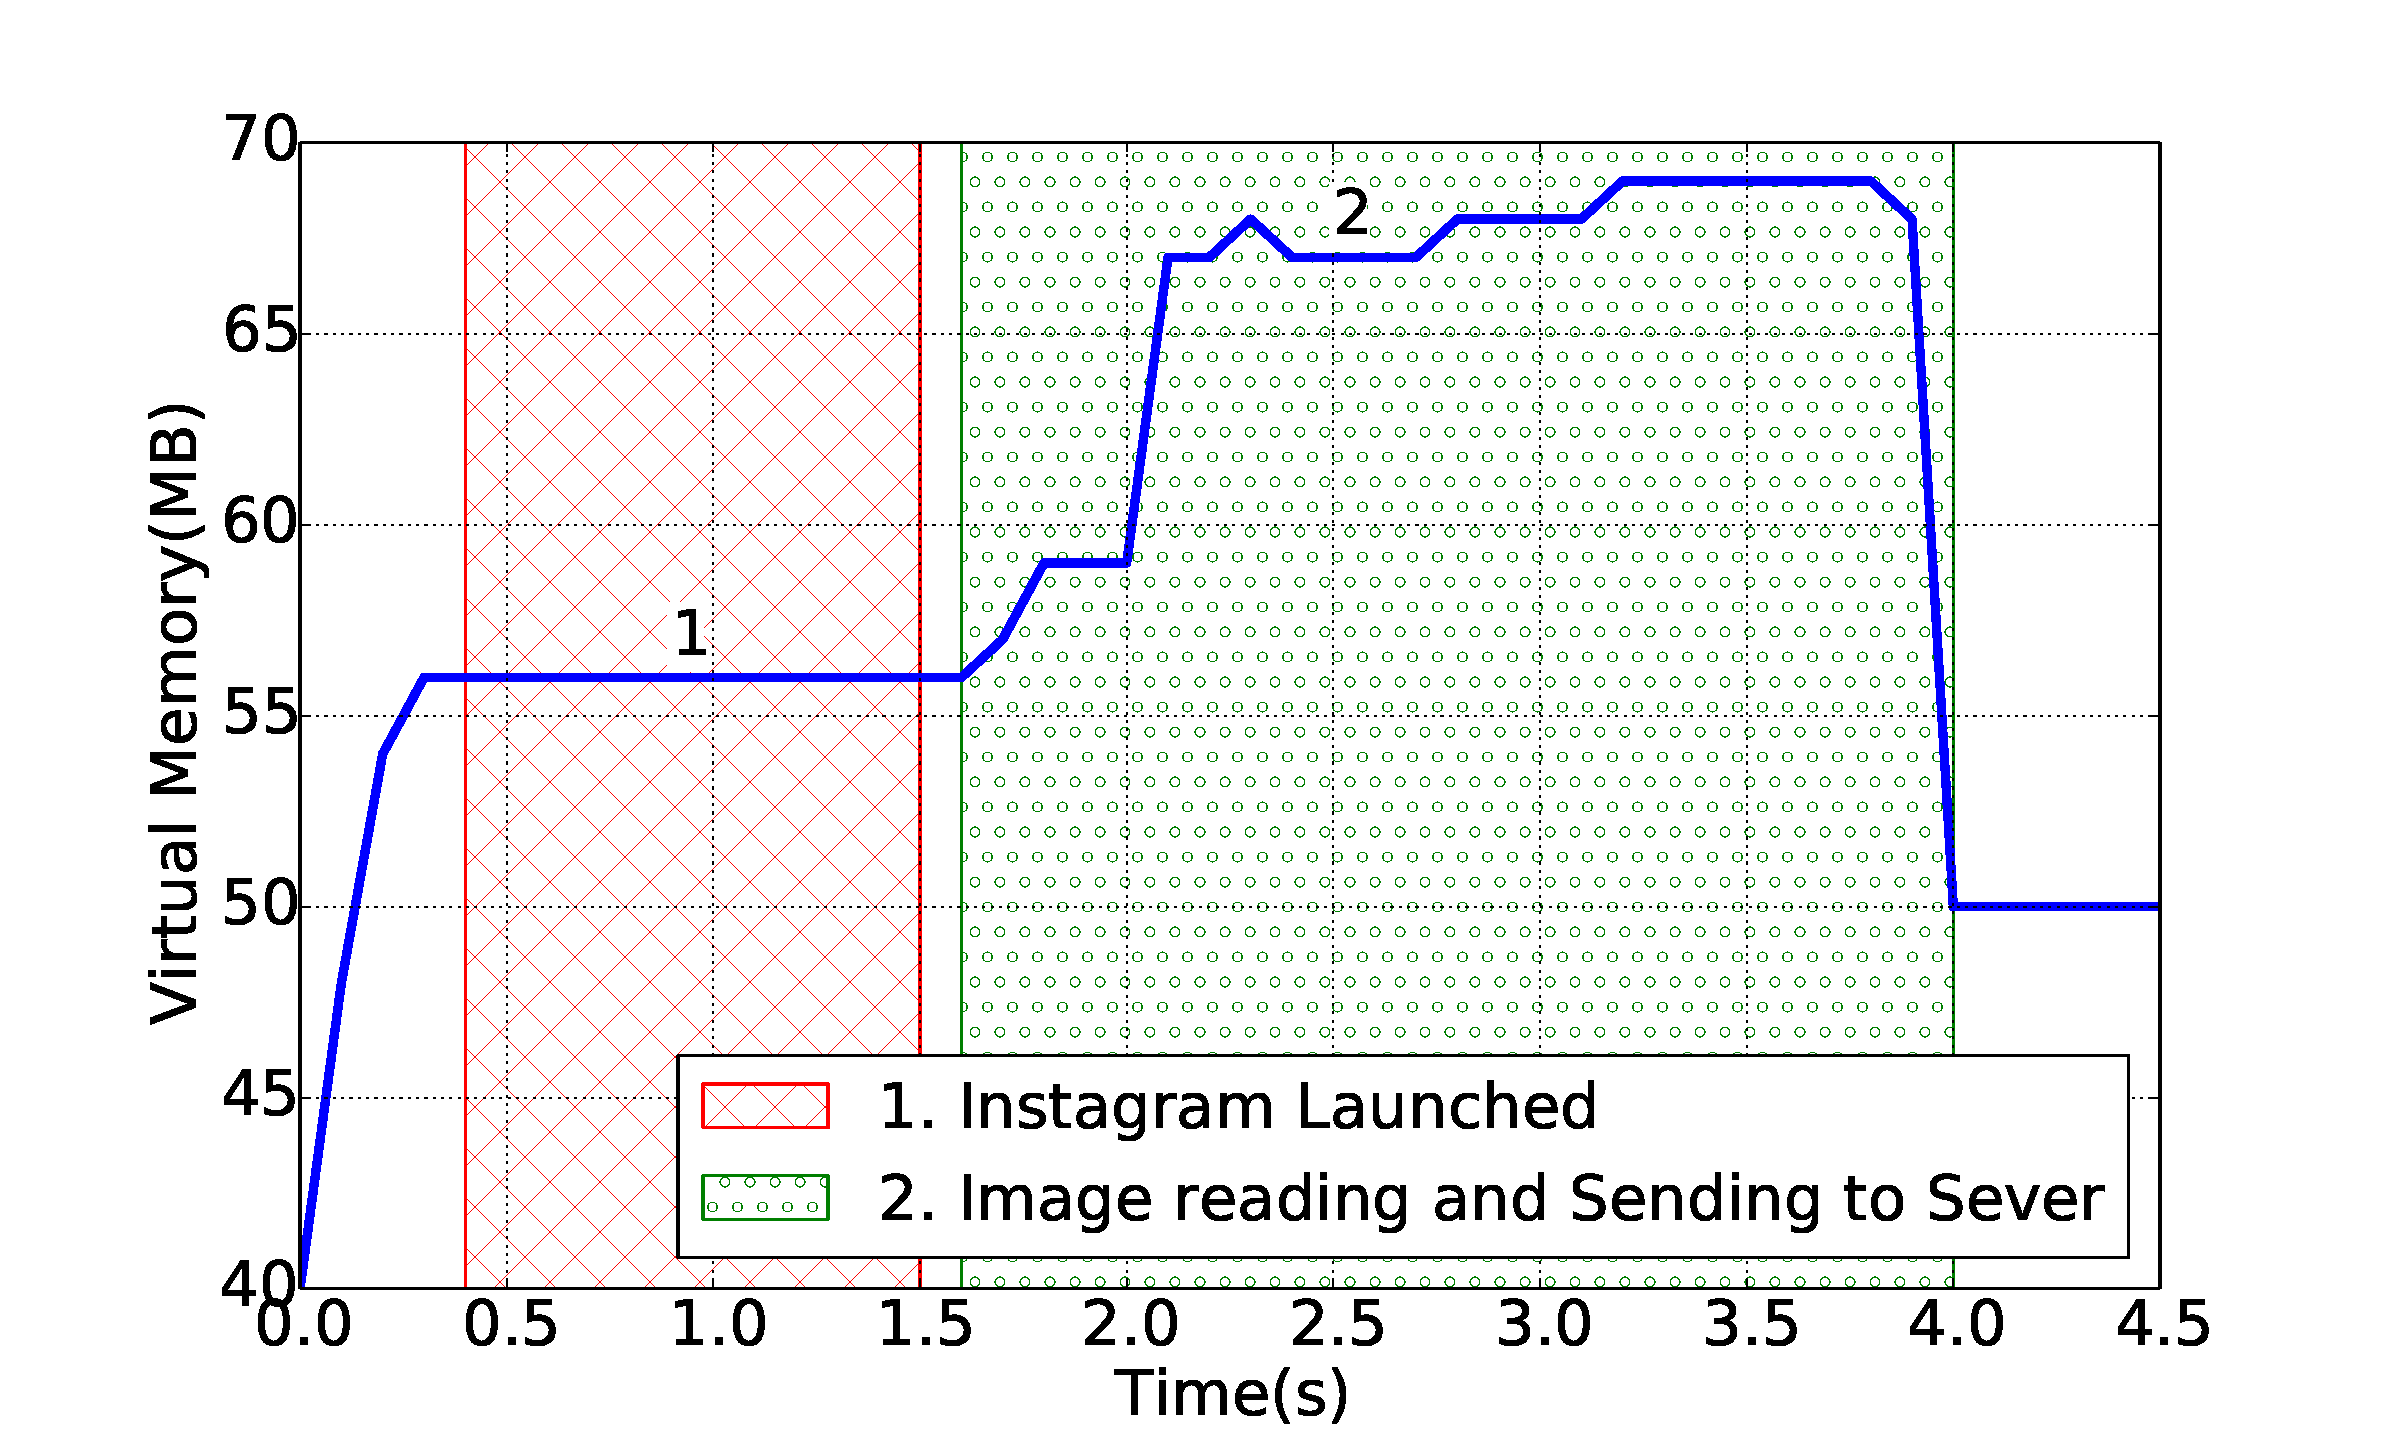
\includegraphics[width=\linewidth]{attack4memory.pdf}
                \caption{Gallery Stealing}
        \end{subfigure}%
        %\quad
        \begin{subfigure}[t]{0.5\textwidth}
                \centering
          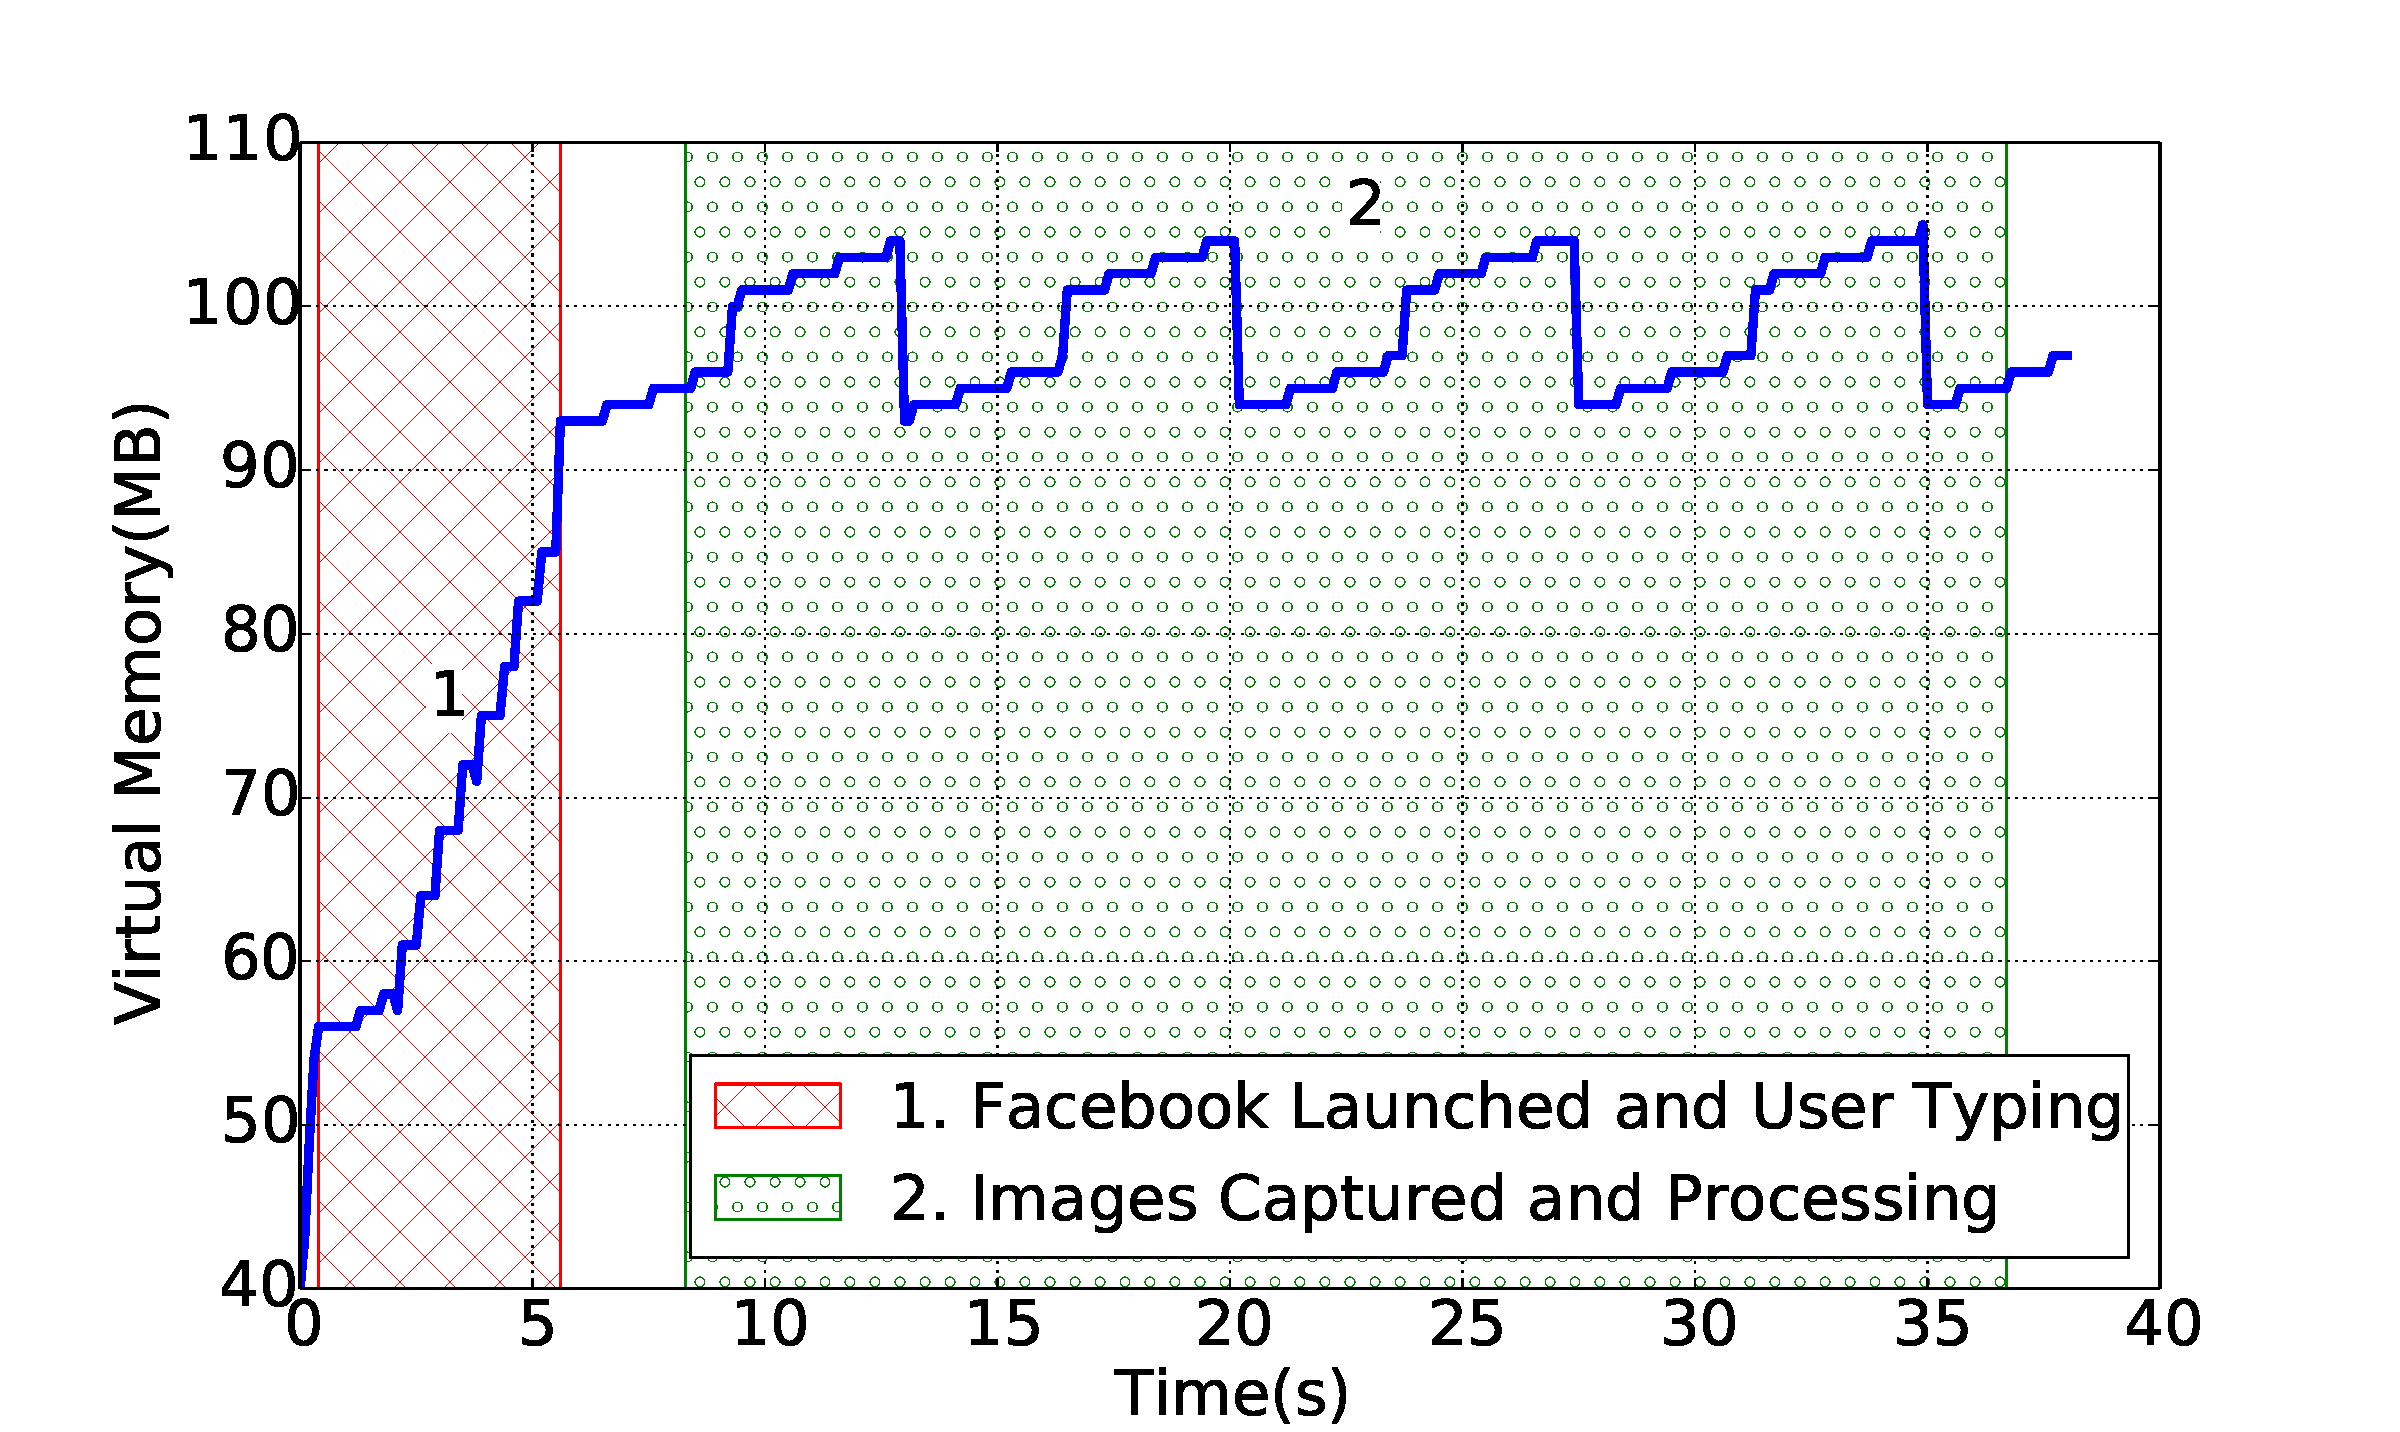
\includegraphics[width=\linewidth]{attack3memory.pdf}
                \caption{Screenshot Capturing}
        \end{subfigure}
         \caption{Memory Distribution Curves}
         \label{fig:memory}
\end{figure}

In addition, we also conduct experiment to monitor the battery consuming
status and evaluate the battery usage of our attacks. The results show
that our attacks may not cause influence on battery aspect (the
battery usage rates of most attacks are $0\%$).  Above all, the
experiment results demonstrate that our proof-of-concept attacks are
light-weight with limited permission requirements.

\subsection{Solutions to Eliminate Task Interference}\label{sec:atmsolution}
In this subsection, we discuss solutions on mitigating Android task
interference. Based on our study, we design and implement a task
interference checking tool to detect the potential risk of task
interference among apps. It protects apps specified by users from
being manipulated by untrustworthy apps. In addition, we also propose
some suggestions to limit the additional privilege achieved by the
apps in the same task.

\subsubsection{Task Interference Checking}
\label{sec:implementation}
In this subsection, we present the design and implementation of our
\textsl{Task Interference Checking} app named \textsl{TICK}.

Based on our understanding of the task interference problem, which
includes the necessary conditions, events and their dependency, we
design a method to check the task interference status among Android
apps.  Table~\ref{tbl:taskinterference} provides us with the basis of
evaluating task interference checking.

\begin{figure*}[t]
        \centering
                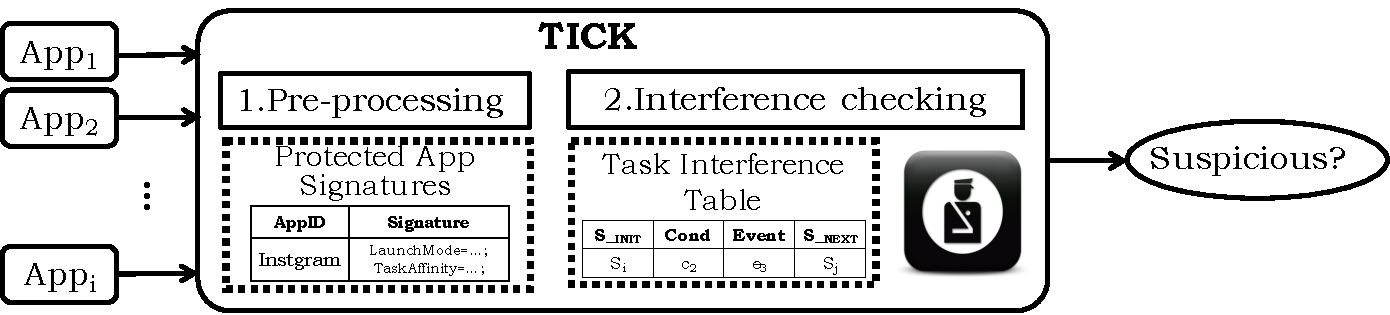
\includegraphics[width=\linewidth]{tick.pdf}
           \caption{Task Interference Checking Architecture}
           \vspace{-0.2cm}
        \label{fig:tick}
\end{figure*}

\textbf{Design.} As shown in Figure~\ref{fig:tick}, \textsl{TICK}
consists of two basic modules, \textsl{Pre-processing} and
\textsl{Interference Checking}, and two supporting databases,
\textsl{Protected App Signature} and \textsl{Task Interference Table}.

\begin{itemize}
\item \textsl{Protected App Signature.} For the apps users who want to
  protect against attacks to Android tasks, this database includes the
  abstracted conditions of such attacks of each app, which is stored as
  signatures in this database.
\item \textsl{Task Interference Table.} This database is the output
  from our research in Section~\ref{sec:atmapproach}, which includes the
  fundamental rules of task interference.
\item \textsl{Pre-processing.} The module takes as inputs the manifest
  files of apps to be checked, abstracts and outputs their task
  interference features for checking.
\item \textsl{Interference Checking.} The interference checking module
  takes inputs from \textsl{Pre-processing} module and \textsl{Protected App
  Signature} database, and checks the suspiciousness of the testing apps
  according to the rules specified in the Task Interference Table.
\end{itemize}

There are two application scenarios for deploying \textsl{TICK}.
\begin{description}

\item[\textbf{C-1:}] Before a user installs an app, she/he can use
  TICK to detect the potential risk of task-related attacks from the app.  TICK
  will parse the app meta data and check with our table and signature
  database to see if it interferes with an existing app. If the app is
  detected to cause interference, TICK will issue a
  warning to the user and suggest she/he not install the app.
\item[\textbf{C-2:}] Our checking app can do chronically scan from
  time to time, check if new packages are added to the device, audit
  if they have security concerns, and notify users if and suspicious
  package were installed.
\end{description}

\textbf{Getting Meta Data of an Activity.}  Currently, our checking app
only considers static declarations of task related attributes from the
app package. Moreover, the key attributes related to Android Task
cannot be altered during runtime, e.g., \textit{taskAffinity} and
\textit{allowTaskReparenting}.

Android SDK provides standard APIs to get an app's Manifest meta data
without requiring any permission. Given a package name and a flag, one
can retrieve an object of \texttt{PackageInfo} through the
\texttt{PackageManager}. Here, we set the flag to
\texttt{GET\_ACTIVITIES} and we retrieve a list of
\texttt{ActivityInfo} by fetching the attribute
\texttt{PackageInfo.activities}. ActivityInfo contains all the meta
data described in the \texttt{Manifest} about every activity of a
package, including those we care, e.g., \texttt{taskAffinity},
\texttt{FLAG\_ALLOW\_TASK\_REPARENTING}, \texttt{LAUNCH\_SINGLE\_TASK}
and so on. The key APIs of getting \texttt{packageManager} and
\texttt{packageInfo} are respectively \texttt{getPackageManager()} and
\texttt{getPackageInfo()}.


\textbf{Effectiveness.} To verify the effectiveness, we used Instagram and our UI-Phishing app
as inputs to TICK. It parsed the meta data of each activity in both
apps and found that most activities of Instagram with {\em
  taskAffinity} set to ``com.instagram.android'', while the rest has
{\em taskAffinity} of
``com.instagram.android.ShareHandlerActivity''. Most of the activities
in Instagram have {\em launchMode} set to ``standard''. A small
portion of the activities have the {\em launchMode} set to
``singleTop'', e.g., the \texttt{LoginActivity}. Very few activities
have {\em launchMode} set to ``singleInstance''. The UI-Phishing app's
first activity has the following flags set: \texttt{taskAffinity =
  "com.instagram.android"}, \texttt{allowTaskReparenting = true} and
\texttt{launchMode = standard}. This matches Case 9 and Case 10 in our
task interference table. When we use TICK to scan the device,
specifying the Instagram app as the one to be protected, TICK
successfully warns users about the potential risk from the UI-Phishing
app. The overhead of TICK can vary based on a number of factors such as device hardware and number of third-party Apps installed in the device. In our experiment, excluding all system-level Apps, there are totally 65 third-party Apps installed in our device. It rougly took 4-5 seconds to scan all Apps and identify suspicious ones.

\subsubsection{Design Suggestions}

From security issues we have demonstrated in the above attacks, it is
clear that the privilege given to apps in the same task is well beyond
what is expected for a mechanism that facilitates app collaboration
and interaction. In fact, the task mechanism should be treated as a
way of {\em authorization}, and the security mechanism around the task
mechanism also should be designed accordingly.

In particular, when treating a task as a boundary for authorization,
we need to be explicit about the ownership of a task and its
authenticity. For example, if an app specifies the {\em taskAffinity}
of an existing task, there needs to be a form of {\em authorization}
before the app can be included into the task, and the authorization
should be carried out by entities with privilege greater than the
privilege given to the task. This is similar to the requirement made
by the UNIX group mechanism. In addition, as the name of ``task affinity''
becomes an identifier for a security object, the system should avoid
name conflicts. In case they occur, they need to be resolved with all
involving entities to avoid unexpected privilege escalation.

\subsection{Related Works}\label{sec:atmrelated}
\textbf{IPC Security:} IPC security is one of the top concerns while
designing OSes. Some early studies have reported security threats in
the Android IPC mechanism. More specifically, Ren
et al.~\cite{TaskHijacking} have proposed the first study of the
security of Android task mechanisms and showed the possibilities of
several enabled attacks, such as back-button hijacking and
uninstalling-prevention attack. Other popular mobile systems like iOS
are also not immune to the risks. Xing et al.~\cite{CrackingiOS}
registered a counterfeit scheme which hijacks the real Facebook scheme
in iOS and successfully stole a Facebook access token that was
supposed to be passed onto the relying-party app. Besides problematic
designs of IPC of OSes, mis-implementation of certain IPC-based
protocols can also lead to security concerns. Chen
et al.~\cite{OAuthDemystified} have conducted an analysis on 149
mobile applications and showed 89 of them (59.7\%) incorrectly
implemented OAuth and thus are vulnerable to SSO-oriented attacks.
Furthermore, IPC vulnerabilities were also documented on other
platforms besides mobile OSes. Take browser platform for an example.
Wang et al.~\cite{webssoattack} discovered 8 serious logic flaws among
the traffics between high-profile ID provider and relying website
through browser platform. Wang et al.~\cite{shopforfree} discovered
logic flaws in several shopping websites and finally purchasing goods
without or with little payment.

\textbf{GUI Security:} As for traditional desktop and browser
environment, GUI security issues have been studied
extensively~\cite{nitpickers,secuserinterface}. Niemietz
et al~\cite{uiredress} implement a UI redressing attacks on Android
devices base on clickingjacking and tapjacking and the attack is
feasible to be transferred from desktop to mobile and to browser,
enabling the attack to be adapted to multiple platforms and
functionalities. As mobile market begins to thrive, GUI security is
more concerned in mobile platforms than ever before. Chen
et al.~\cite{UIstateinference} managed to impose Hidden Markov Model
(HMM) on a public resource \texttt{shared\_vm} combining a bundle of
data to perform UI Inference Attack and successfully stole sensitive
information from users such as user names, passwords and check images.
Wang et al.~\cite{jekyll} implemented a malicious app which
circumvented the Apple Code Review system and successfully stole user
secrets stealthily. 

\textbf{Defending against Malicious Behaviors:} Defending malicious
behaviors can be categorized into two branches, detection and
prevention. In previous studies, various detection schemes have been
introduced to prevent GUI-related attacks. Fu
et al.~\cite{detectpswebsite} employ the Earth mover's distance (EMD)
mechanism to detect possible malicious web page through measuring the
similarity between two web pages by first converting web pages to
images, and then grabbing and comparing the feature points through
training data set. More generally, Chen et al~\cite{peg} introduce the
concept of permission event graph (PEG) with model checking mechanisms
to detect abnormal behaviours of Android apps. As for prevention, one
idea is to prevent sensitive data from being leaked to the malicious
server party. Hornyack et al.~\cite{AppFence} develop a
system for Android called AppFence, which can block the sensitive data
from being transmitted, or substitute the fine-grained data to
coarse-grained data if transmission is unpreventable. Ren
et al.~\cite{Windowguard} develop WindowGuard which protect against GUI
attacks by enforcing the Android Window Integrity (AWI).

   \newpage
   \begin{singlespace}
   \section{xxx}\label{sec:dssnassociate}
   \end{singlespace}

%==========================================================================================================================
\section{Conclusion and Future Work}\label{sec:conclusion}

xxx


        \newpage
   \bibliographystyle{abbrv}
   \bibliography{proposal}
\end{document} 